\documentclass[11pt]{article}
\usepackage[affil-it]{authblk}
\usepackage{graphicx}
\usepackage[space]{grffile}
\usepackage{latexsym}
\usepackage{textcomp}
\usepackage{longtable}
\usepackage{multirow,booktabs}
\usepackage{amsfonts,amsmath,amssymb}

% You can conditionalize code for latexml or normal latex using this.
\newif\iflatexml\latexmlfalse
\usepackage[utf8]{inputenc}

\usepackage[left=40mm,right=20mm,top=20mm,bottom=30mm]{geometry}
\usepackage{natbib}
\usepackage{booktabs}
\usepackage{endnotes}
\usepackage[toc,page]{appendix}
\usepackage{pdfpages}
\usepackage{graphicx}
\usepackage[parfill]{parskip}
\usepackage{url}
\usepackage{breakurl} 
\usepackage[breaklinks]{hyperref}

\bibliographystyle{abbrvnat}

%\usepackage[style=authoryear-ibid]{biblatex}
\setcitestyle{authoryear-ibid,open={(},close={)},citesep={;},aysep={,}}
%\setcitestyle{authoryear,open={(},close={)}}
\linespread{1.5}

%\usepackage[UKenglish]{babel}

\usepackage[nottoc]{tocbibind}
\usepackage{caption}

\begin{document}
	
\includepdf{CoverSheet}
\includepdf[pages=-]{Ethics}
\includepdf[pages=-]{Summary}


\begin{titlepage}

		%titlepage
		\thispagestyle{empty}
		\begin{center}
			\begin{minipage}{0.75\linewidth}
				\centering

				\includegraphics{mdx.png}\\
%				\rule{0.4\linewidth}{0.15\linewidth}\par
				\vspace{3cm}
				%Thesis title
				{\uppercase{\Large Pushing the Boundaries: An Investigation into a Focus on Innovation within an Education System\par}}
				\vspace{3cm}
				%Author's name
				{\Large Kieran Hogg\par}
				\vspace{3cm}
				%Degree
				{\Large A thesis submitted in partial fulfilment of the requirements for the Masters in Education Degree\par}
				\vspace{3cm}
				%Date
				{\Large September 2016}
			\end{minipage}
		\end{center}
		\clearpage
\end{titlepage}
\begin{abstract}
	
A truly innovative education system is highly sought after by most countries. Evidence of this can be seen by the amount of focus the Finnish system received after diverging from global education policies which resulting in performing unexpectedly well in the global PISA assessments for much of the 2000s.

In the 2015-16 academic year, a unified inspection framework was published for schools in the United Arab Emirates. Uniquely, innovation was included as area which schools would be directly measured. This was a new explicit measurement of education, both in the UAE and globally.

As an abstract concept within the field of education, this research investigates the understanding of innovation, what changes, if any, have been made in reaction to the ostensible promotion and measurement of innovation within schools.

Using a pragmatic approach comprising qualitative and quantitative data collected via surveys from teachers, interviews with school leadership and observational case studies, the research has aimed to collate differing perspectives of innovation with the aim of contributing to a more inclusive definition.

The research demonstrated that innovation as a concept in the UAE education system is a dynamic process that continues to evolve and develop as it moves from its infancy to a more mature concept. The discovery of an innovation skills guide, for example, which was otherwise unpublished and not disseminated among institutions, served to show that not all practices were known to institutions with regard to how innovation was marked or measured.

Through the case studies, commonalities and good practice of innovative schools, the data gives a clearer picture of how schools use innovation, put the concept into practice and what factors enabled them to do so. They also discussed what benefit innovative schools have on students, teaching in particular.

\end{abstract}

\newpage

\tableofcontents



\newpage%

\section{Chapter 1}
\subsection{Introduction, Focus and Overview}
Innovation is a word and concept most are familiar with. The term itself is applicable to almost every industry and is in common usage, both in spoken, written and as a consistently popular search term on the internet \citep{CorpusofContemporaryAmericanEnglish,Google}. It is not, however, a buzzword. As seen in Figure \ref{fig:popularity}, the subsequent popularity of innovation according to Google Trends, and the popularity of the term has remained fairly constant since 2004.

\begin{figure}[h]
\centering
	\captionsetup{justification=centering}
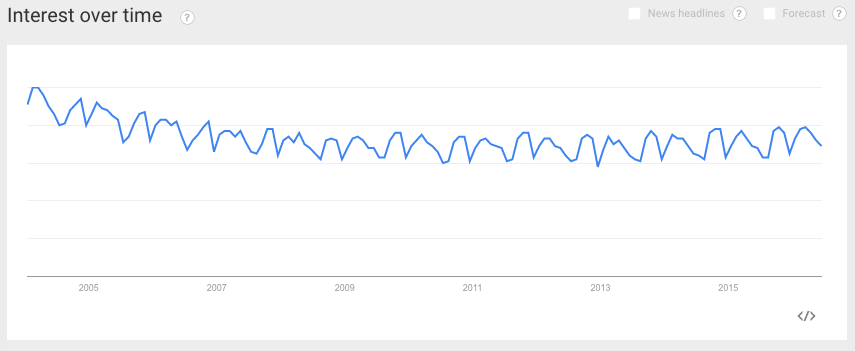
\includegraphics[scale=0.53]{figures/Innovation searches/Innovation searches_original}
\caption{Popularity of the search term `innovation' over time according to Google Trends\citep{Google}}
\label{fig:popularity} 
\end{figure}

In the 21st century, for most people, innovation conjures images of technology and the Internet. Unsurprisingly, the most closely-related phrase according to Google is `technology innovation' \citep{Google}. The increase in prevalence of home technology and access to the Internet would rightfully be the most common example of innovation in recent times. A close second is `business innovation' which is a context where the word `innovation' is commonly used in conjunction with, and where companies such as Apple, Google and Facebook are combining those two areas to outstanding success.

However, one of the areas perhaps not as traditionally thought of as being innovative is education. The idea of an educator who holds the knowledge and dictates that to students has changed somewhat over the last hundred years, but the core idea of that is still seen in most classrooms even today. 

Those more familiar with educational developments will appreciate that while this is true, there have been, and continue to be, many changes and innovations that take place within education; it is by nature a dynamic profession and environment. Some of recent educational changes include the three-part lesson which has been introduced and has remained prevalent; learning styles became popular and are now on the way out \citep{coffield2004should} and personalisation along with a better understanding of SEN students has been a huge positive development for the better.

At any given time, there are numerous entities researching and implementing different ideas and changes in education, some hugely innovative, some less so. Sometimes the impetus for change comes from research institutions, governments, sometimes from schools, sometimes from teachers or occasionally, from other agents such as parents and students. 

This research will focus on an aim to produce a more innovative education system in the United Arab Emirates, introduced by the UAE government.

The United Arab Emirates is one of the fastest developing countries in the world (see Figure \ref{fig:population}) which having only been established in 1971, is developing its public and private sectors at a rapid rate to match the influx of people migrating to the country. Education is no exception to this, with an increase in both non-local educators and workers in other sectors bringing their children to be educated in the country. This has led to an education system which is both rapidly developing to try to catch up with that of much older countries, but also one which does not have the history and baggage. 

\begin{figure}[h]
	\centering
	\captionsetup{justification=centering}
	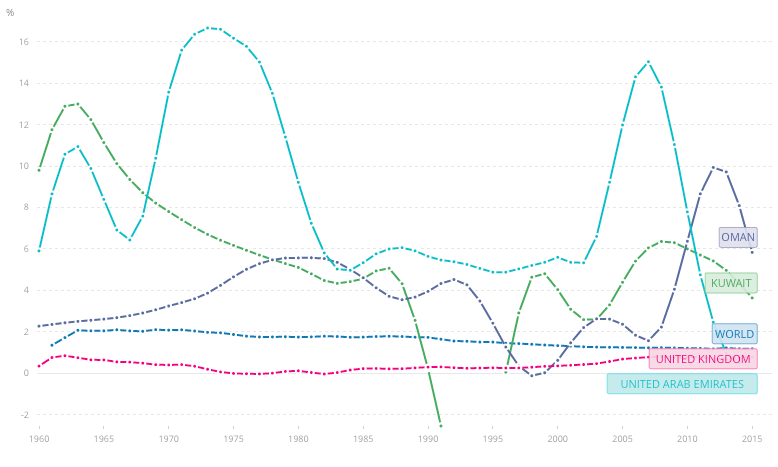
\includegraphics[scale=0.6]{figures/population}
	\caption{Population the United Arab Emirates from 1960 to 2015, relative to other countries \citep{worldbank}}
	\label{fig:population} 
\end{figure}

The UAE comprises seven emirates. The largest and home to the nation's capital city is Abu Dhabi. Schools in Abu Dhabi come in two main forms: the first is public schools, which offer free education to mainly Emirati children (expats must be under 20\% of the school, speak Arabic and pay tuition fees) and offer either an Abu Dhabi Education Council (ADEC) or Ministry of Education curriculum depending on the type of school. Private schools make up the remainder. These are fee-paying and typically follow a foreign curriculum such as British, American or Indian. While private schools are more independent in their operation and curriculum, ADEC still has a role in inspecting these schools to ensure overall quality and compliance across the emirate. They are also increasing in both number, and in popularity. To put private school attendance into context, in 2011 87\% of students in Dubai were attending a private school, 56.7\% of which were Emirati students \cite[p.16]{Kenaid2011}. When surveyed, 50\% of parents indicated the main reason as `better quality teaching and learning'.

At the start of the 2015-2016 academic year, a unified inspection framework for schools in the UAE was published after collaboration by education authorities for the country. Participating organisations and regulatory bodies included ADEC; the Knowledge and Human Development Authority (KHDA); the Abu Dhabi Centre for Technical and Vocational Education and Training (ACTVET) and the UAE Ministry of Education. One of the new additions to the framework, which otherwise looks broadly similar to that of most developed countries, was the addition of innovation as an additional focus. To put it into perspective, innovation is given comparatively the same amount of weighting in the framework as more established educational concepts such as inclusion. ADEC discusses innovation as follows:

\begin{quote}
	Innovation comes in many forms. There are innovations in the way schools are owned, organised and managed; in curriculum design models; in teaching and learning approaches, such as the ways in which learning technologies are used; classroom design including virtual spaces; assessment; timetabling; partnerships to promote effective learning and engagement in the economy; and the ways in which teachers and leaders are recruited, trained, developed and rewarded. These innovations can be small or large, recognisable or entirely new and different.
	
	Innovation is driven by a commitment to excellence and continuous improvement. Innovation is based on curiosity, the willingness to take risks and to experiment to test assumptions. Innovation is based on questioning and challenging the status quo. It is also based on recognising opportunity and taking advantage of it. Being innovative is about looking beyond what we currently do well, identifying the great ideas of tomorrow and putting them into practice.
\end{quote} \cite[p.12]{ADEC2015}

The idea of innovation in education is not a new one, but its prominent position in an inspection framework indicates the importance that the government is placing on innovation for the education system. Indeed, the framework makes reference to the UAE Vision 2021 as justification to the inclusion of innovation as an educational focus. There are many references to innovation in the vision, but the clearest one states: ``We want the UAE to transform its economy into a model where growth is driven by knowledge and innovation" \citep{UAEGovernment2012}.  The importance placed in this area, the slightly surprising inclusion and the lack of exposure to it were the driving factors for choosing this as an area to focus on.

Hypothetically I think that there will have been some good work from schools so far but that how schools have interpreted it and implemented it so far will differ. That is not to say that this is a bad thing; one of the hopeful outcomes of this research is a clearer picture which will enable other educators to learn from others.

I think the difference in implementation will be a reflection of the diversity present in education in the UAE with various different types of educational establishments, staffed by many different nationalities, which are all at different stages of their educational lives.

Broadly speaking, the initiative will be examined in the following ways: 

\begin{itemize}
	\item What is innovation in education and what is the goal of the initiative?
	\item What form of innovation has taken place in schools so far?
	\item How consistent is the interpretation of innovation between schools across the region?
	\item How do the above answers compare to a more developed educational system?
	\item Has there been any impact so far? What is the predicted future impact?
\end{itemize}

\subsection{Needs Analysis and Justification}

The need for this research varies from party to party. The common need for  all is to provide some clarity and context in the first instance. As a relatively new and novel (at least as an assessed outcome) focus, there is still some uncertainty surrounding it.

As a teacher within an Abu Dhabi school, there are a few different needs that may be satisfied by this research. With innovation seemingly playing a large part in the future educational landscape in Abu Dhabi and the UAE, as a teacher I would like to be as informed about it as possible. As there is not an immediate wealth of information regarding how I should go about it as a classroom practitioner, this will aim to fill that immediate need.

As part of a team, the need is not only to provide some best practices but to provide some context and evaluation of what we and other establishments are doing within the local area. There will be some examination and scrutiny over initiative that are already in place as to their effectiveness.

More broadly, the innovation focus has been seemingly added as a reaction to a deficit to improve the education system in certain areas. The UAE is aiming to bring its educational system up to the highest global standards as they have done so in other areas of society successfully. This is not done in a vacuum however, and this research will look at the origins, process and possible goals in creating an innovative educational system. While not common, it is not without comparison, so by analysing it with a global and historical perspective, any successes and challenges may be able to be inferred from other nations and other initiatives worldwide.


\subsection{Professional Autobiography}
My educational background has always been heavily focused around computers and technology. My secondary education took in A-Level ICT and Computing, which naturally led me to a degree in Computer Science. During my degree I was fortunate to work for a software company for a year full time and a further year part time. This was followed by a PGCE in ICT.

Upon my qualification, ICT qualifications taught in England were still very prescriptive and based around the teaching of Microsoft Office skills. As a result of my background, I felt naturally inclined to innovate with technology and the curriculum where it allowed. As a result, I believe that innovation is not solely the use of technology in the classroom in and of itself. I believe it can be a useful part of an innovative approach when used correctly, but simple use of technology is not innovation. 

To give a practical example, the use of interactive white boards is still something on which new staff receive training and is discussed as being used innovatively. Perhaps surprisingly, white boards were developed in 1990 and by 2007, 98\% \citep{kitchen2008harnessing} of secondary schools had them in every classroom. Given their age and ubiquity, the use of white boards cannot and should be considered as innovative practice. They do however, offer a positive example of a technological innovation improving teaching and learning, having become such a mainstay in modern classrooms.

My natural inclination therefore is to see innovation within education as holistic rather than one particular idea. This will obviously affect my initial opinion but will have no effect on the analysis of the data relating to how other teachers view it.

The use of technology has always come naturally so my inclination has always been to pursue technology in an effort to make my teaching and learning either easier, or more engaging. The reason for innovation and technology becoming almost synonymous in technology is twofold: a lot of technology can be genuinely innovative and can be `easy win' with its prevalence and impact, and secondly for many teachers, technology is the most obvious way to innovate within the classroom.

My interest in the topic is comprised of a few different angles of personal relevance. I currently work in a new school which is not only innovative at present, but has many innovative plans for the future. I am keen to see innovation as a driving force for change in schools rather than as a tick box used during inspections. During my career I have had the opportunity to observe and work with many innovative projects, both technological and otherwise. Some have worked, some have not, as is the case for the innovation process. The projects based around technology have proved to be useful lessons from the perspective of someone with a great interest in the area. With the focus on innovation being so prominent, I am keen to be able to find similar examples in the local area to collate and share within this research.

Teaching is both an amazingly collaborative profession and an incredibly individual profession. The collaborative nature is evidenced by the amount of resources online and the rich personal learning networks that have emerged on platforms such as Twitter. In contrast, anyone who has written a lesson plan from scratch rather than use one that has been written by another teacher will understand this strange dichotomy. One of the hopes of this research is to share some best practice in this area.

To mitigate the potential personal bias for these areas, I will be ensuring the majority of data and conclusions are drawn from sources that are not my own. To the greatest extent possible, questions will be written in a neutral and open way to prevent any leading questions.

As an employee in a school, I may be inclined to have bias towards my institution's direction and practice. There must be a certain amount of critical thinking towards innovative practices however, but any side-by-side comparisons will be limited to good practice to ensure that these biases do not appear in the form of diminishing others’ achievements and our shortcomings. 

Valid areas of criticism of the innovation drive will be drawn out from staff at their institutions to ensure the analysis is as fair as can be achieved. The research is looking to tell both sides of the story with the implementation.

Due to my location and employment, the research will be mainly based in Abu Dhabi and Dubai private education. For national context, Dubai is the leader of UAE education with scores slightly above the PISA average \citep{2013}. The remaining emirates are below the PISA average, with Abu Dhabi coming in third below Sharjah \citep{2013}. Within the timescale of the research, it would not be possible to do a country-wide investigation. Therefore, some of the findings and conclusions may well not be applicable to the current timeline in the northern emirates, but it is hoped that even though it may not currently apply, many of the findings will be still be relevant given the innovation drive is a national one.
\section{Chapter 2}
\subsection{A Critical Review of the Literature}
One of the first challenges when approaching a review of the literature is to be able to define the scope of the literature search. In order to be able to accurately discover appropriate material, we must attempt to define innovation within the context of education. Given the simplicity of the term and the complexity of the meaning and implications, it comes as no great surprise that there is not a singularly accepted definition. The best attempt to define it using the range of related definitions found during the review is the following collective definition by \citet{Sharma_2005}:

\begin{quote}
	The variety of ways in which the concept of innovation has been defined by researchers reflects the nature of the discipline (Gopalakrishnan, 1994), the level at which innovation is conceptualised, and whether it is being conceived as a product or process (Amabile, 1988; Kanter, 1988). According to one of the earlier definitions, innovation is an idea, practice or material artefact perceived to be new by the relevant unit of adoption (Allen, 1975). Later, Anderson and King (1993) conceptualised innovation as the emergence, import or imposition of new ideas which are pursued towards implementation, through interpersonal discussion and successive remoulding of the original proposal over time. This contemporary definition not only describes the nature of innovation, but also refers to the intrinsic process of implementation. With advances in research, the concept of innovation has also been refined and a more comprehensive understanding of innovation has emerged. It may be defined as the introduction and application within a group, organisation, or wider society, of processes, products or procedures new to the relevant unit of adoption and intended to benefit the group, individual or wider society (West \& Farr, 1990)
\end{quote}

This a more general definition than one would normally come across specifically in education, but it helps to give the full context of the derivation. The distinction of innovation being considered both as more than one aspect as well as a combination of other aspects is one that will be discussed further.

A slightly narrower definition, although one that is probably more fitting for an educational context is where innovation is differentiated from improvements by the notion that innovation is ``planned deliberate change ... but it does not necessarily result in [enhancement]." \citep{hannan2002innovative}

With this innovation drive, there seem to be three main areas of primary focus: creating an innovative education system; developing innovative schools and teaching students to be innovative. Those areas were looked at as part of the literature review, as well as a few other areas which seemed of relevance.

\subsubsection{Innovative Education Systems}
The aim of this entire project is to enable the UAE's schools to be more innovative, to create more innovative students who will in turn become more innovative citizens in order to further the overall goal of a more innovative country, industry and economy. While the enthusiasm over the last few years \citep{1_sahlgren_2013, 2_clark_2016, 3_anderson_2016}, Finland is still held up as an education system which radically transformed itself and became the go-to example for an innovative education system.

There are many studies on how and why Finland has managed to get to where it is now, one study tries to demonstrate this by highlighting some of their educational principles, shown in Table \ref{finnish-policies}.

\begin{table}[]
	\resizebox{\textwidth}{!}{%
		\begin{tabular}{@{}ll@{}}
			\toprule
			\multicolumn{2}{c}{Education policies and reform principles}                                                                                                                                                                                                                                                                                                                                                                                                                                                                                                                                                                                                                                                                                        \\ \midrule
			Global education reform trends                                                                                                                                                                                                                                                                                                                                     & Education policies in Finland                                                                                                                                                                                                                                                                                                                                                  \\ \bottomrule
			
			\begin{tabular}[c]{@{}l@{}}\textbf{Standardization}\\ Setting clear, high and centrally prescribed\\ performance standards for schools, teachers\\ and students to improve the quality of\\ outcomes.\end{tabular}                                                                                                                                                          & \begin{tabular}[c]{@{}l@{}}\textbf{Flexibility and loose standards}\\ Building on existing good practices and\\ innovations in school-based curriculum\\ development, setting of learning targets and\\ networking through steering by information and\\ support.\end{tabular}                                                                                                          \\
			\begin{tabular}[c]{@{}l@{}}\textbf{Focus on literacy and numeracy}\\ Basic knowledge and skills in reading, writing,\\ mathematics and natural sciences as prime\\ targets of education reform.\end{tabular}                                                                                                                                                                & \begin{tabular}[c]{@{}l@{}}\textbf{Broad learning combined with creativity}\\ Teaching and learning focus on deep and broad\\ learning giving equal value to all aspects of an\\ individual’s growth of personality, moral,\\ creativity, knowledge and skills.\end{tabular}                                                                                                            \\
			\begin{tabular}[c]{@{}l@{}}\textbf{Consequential accountability}\\ The school performance and raising student\\ achievement are closely tied to the processes of\\ promotion, inspection and ultimately\\ rewarding or punishing schools and teachers\\ based on accountability measures, especially\\ standardised testing as the main criteria of\\ success.\end{tabular} & \begin{tabular}[c]{@{}l@{}}\textbf{Intelligent accountability with trust-based
					professionalism}\\
				Adoption of intelligent accountability policies and\\ gradual building of a culture of trust within the\\ education system that values teachers’ and\\ headmasters’ professionalism in judging what is\\ best for students and in reporting their learning\\ progress.\end{tabular} \\ \bottomrule
		\end{tabular}%
	}
	\caption{A comparison of Finnish and global educational policies \cite{Sahlberg2007}}
	\label{finnish-policies}
\end{table}

Many of the global education systems have found it difficult to emulate the Finnish model as it tends to go against most of the modern trends in education. As shown in Table \ref{finnish-policies} Finnish policies are contrasted with the corresponding global trends. Anyone who has taught in a school in America, Europe or many other countries will recognise the global set of policies as the norm in education systems. Is it therefore possible the UAE could be more successful than others in its attempts to become an innovative educational system? Due to their relative youth of their educational system, they have not typically followed the global trends as closely as other countries have.

Commentators \citep{Hatherley-Greene2016} argue that the UAE and the Finnish model are incompatible due to the differing social constructs, based on models from 1970s that indicate Finland to be very much more independent and egalitarian. Comparing the following, there are definitely similarities:

\begin{quote}
	Emiratis tend to accept a social hierarchy and deference to figures of authority. The UAE is a collectivist society in that its members strongly associate themselves with the larger community, sometimes subsuming their personal wishes for the greater good of the group.
\end{quote} \citep{Hatherley-Greene2016}

\begin{quote}
	Traditional values have endured [in Finland], these include such cultural hallmarks as a law-abiding citizenry, trust in authority, commitment to one’s social group, awareness of one’s social status and position, and a patriotic spirit.
\end{quote} \citep{Sahlberg2007}

This is echoed elsewhere: ``It could be said, even at the risk of accusations of speculation, that Finnish culture still incorporates a meaningful element of the authoritarian, obedient and collectivist mentality" \citep{Simola2005}.

The relatively late and rapid development of Finland, is also a process which mirrors the UAE albeit has had a slight head start:

\begin{quote}
	The late process of industrialization and the simultaneous growth of the service sector brought an exceptionally rapid structural change in society. The transitions from an agricultural to an industrial society, and further to a post-industrial society, have taken place within such a short period of time that one could almost say that these societies currently co-exist in a very special way in the country.
\end{quote} \citep{Simola2005}

The countries outwardly appear to be at least superficially similar which could lead to an innovative drive in education being successful. There are of course significant differences between the two countries. Finland has previously had an extremely homogenous population, whilst migration into Finland has rapidly increased over the recent years, its rate of residents who speak a language other than Finnish is 5.4\% from a population of 5.2 million \citep{OfficialStatisticsofFinlandOSF2011}. The UAE by contrast has an estimated 1.4 million Emiratis \citep{HABBOUSH2013}from a population of 9.2 million \citep{MalitJr.2013} giving an 85\% rate of expats in the country.

\subsubsection{Innovation Studies}
Innovation Studies is an Icelandic subject which appeared in 1999, and was introduced to their national curriculum from 2007. On first reading, a subject related to Design and Technology would not appear to hold much relevance to the broader idea of innovation aside from sharing the name. Reading the emphasis behind it however, it becomes clearer as to the similarities:

\begin{quote}
[Innovation Studies] is driven by an innovation process rather than subject content and as such is cross-curricula. Students capitalize on their knowledge from all sources. In addition, innovation exercises can provide a context for researching an further understanding. 
\citep{thorsteinsson2005innovation}
\end{quote} 

This form of innovation is therefore as a subject; a set of skills which students are allowed to develop and practice in order to become innovative students. They had also identified a subject with which to build it in to, or to develop, that being Design \& Technology.

This is an interesting facet of innovation given the other non-subject forms of it are much more common, in practice and in the literature. This will be an interesting comparison in terms of how this related to teaching of student skills, whether it can be focused in a particular area or whether they need be more cross-curricular.

\subsubsection{Innovation Within Schools}
One of the more in-depth studies is a study focusing on a wide range of areas within Israeli schools \citep{tubin2003domains}. They devised a series of aspects on which they assessed each school, ultimately producing a score for the average level of innovation in each school. The schools were scored on:

\begin{itemize}
	\item Physical space - use (or not) of the traditional classroom
	\item Digital space - use of any technological `space' such as a VLE (Virtual Learning Environment)
	\item Time - whether this was taking place within traditional lessons, virtual courses etc.
	\item Student roles - developing the roles that students take within the classroom such as teaching assistants
	\item Teacher roles (with students and teachers) - if teachers took on differing roles in the classroom and working with colleagues
	\item Curriculum content - use of innovative techniques to enrich or change existing curricula
	\item Didactic solutions - the movement away from traditional didactic approaches such as paper-based worksheets
	\item Assessment methods - primarily the use of ICT to develop new or facilitate exiting assessment practices
\end{itemize}

The use of scoring to come up with an average innovation score is quite an interesting concept and the foci would seem to be a selection which most people could agree an innovative school would have some of them present. Where the study does reveal its age is the loose relationship of ICT equalling innovation; ICT is mentioned in the majority of areas discussed, with a comment on one school's innovative curriculum content stating that ``the French language teacher asked her students to find their favourite French songs and food on the Internet to enrich their own Website". While this is good example of a cross-curricular lesson, this would not pass for innovation any longer.

Whilst Tubin et al. took a all-encompassing look at the school environment, there are more studies which look at innovation within the management, culture and leadership of schools. One of the broader of these, but still with a focus on the process rather than the output, is \citet{Sharma_2005} which proposes a framework to maximise the impact of innovation within schools, an interesting finding being ``that innovations in schools are not resource intensive". Their devised framework is:

\begin{itemize}
	\item Leadership
	\begin{itemize}
		\item Support and Encouragement
		\item Networking
		\item Openness in Communication and Team Effort
	\end{itemize}
	\item Review and Monitoring
	\item Mobilising Community Support
	\item Creating Linkages - Far and Wide
	\item Teachers' Selection, Training and Growth
	\item Decentralised and Participative Management
	\item Smooth Vertical and Horizontal Communication
	\item Emergence of Processes and Systems Unique to the Respective Schools
	\item Institutionalisation of Systems and Procedures
\end{itemize}

This is interesting to compare and contrast this framework with ADEC's own areas, with a reasonable amount of crossover:

\begin{itemize}
	\item the way schools are owned, organised and managed; 
	\item in curriculum design models; 
	\item in teaching and learning approaches, such as the ways in which learning technologies are used; 
	\item classroom design including virtual spaces; 
	\item assessment; 
	\item timetabling; 
	\item partnerships to promote effective learning and engagement in the economy; 
	\item and the ways in which teachers and leaders are recruited, trained, developed and rewarded
\end{itemize}

Sharma et al. have gone one step further than Tubin et al. by taking both a wider look at the environment that must be present for innovation to happen, as well as abstracting them into a set of principles which can be used as a framework for schools who wish to be innovative. In the absence of any guidelines set forth as to the notion of innovation, these two studies initially look like a good starting point for the investigation into the local schools and level to which they are being innovative.

\subsubsection{Innovation Within Other Establishments}
Innovation is an idea that has an application in almost any context. Research into innovation outside the sphere of education is certainly prevalent, and the publications discussed are those that have been identified to have some parallels or application with the target context of schools.

One of the seminal works on innovation in business is \citet{nonaka1995knowledge}. It is a wide-ranging and in-depth look at the idea that Japanese companies were (in the 1990s) seen to be extremely innovative by Western observers. The breadth is far too extensive to detail and while there is some relevance to this study, the majority is understandably business-focused. While some schools are businesses too, they are unique in that their product (delivery of knowledge) is in the majority of cases, free at the point of delivery.

The core of the study focuses on tacit and explicit knowledge; how it is used and transferred:

\begin{quote}
	...[this is] a shared understanding of what the company stands for, where it is going, what kind of world it wants to live in, and, most important, how to make that world a reality. In this respect, the knowledge creating company is as much about ideals as it is about ideas. And that fact fuels innovation. The essence of innovation is to re-create the world according to a particular vision or ideal. To create new knowledge means quite literally to re-create the company and everyone in it in a non-stop process of personal and organizational self-renewal. In the knowledge-creating company, inventing new knowledge is not a specialized activity – the province of the R\&D department or marketing or strategic planning. It is a way of behaving, indeed a way of being, in which everyone is a knowledge worker – that is to say, an entrepreneur.
\end{quote}

The so-called `knowledge-creating' company is based on the `spiral of knowledge' shown in Figure \ref{fig:spiral}. On reading, there is an inescapable context of product creation, invention and entrepreneurship. If that can be overlooked however, the knowledge transfer idea is a generic idea which could be applied to almost any organisation.

\begin{figure}[h]
	\centering
	\captionsetup{justification=centering}
	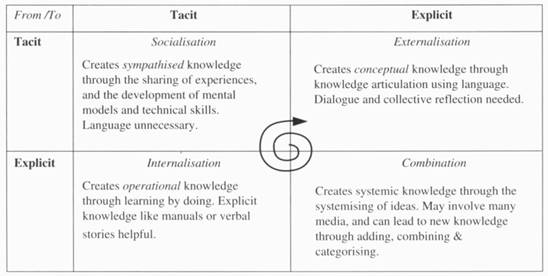
\includegraphics[scale=0.6]{figures/spiral}
	\caption{The SECI cycle of knowledge creation, image by \citet{Hyman} adapted from \citet{nonaka1995knowledge}}
	\label{fig:spiral} 
\end{figure}

When thinking about schools in relation to this idea, there quickly appears the separation between teaching, teachers and students, and management, organisation and leadership. Teaching is a classic example of traditionally tacit information; teacher training definitely has explicit information such as standards and frameworks but a large part is observing, shadowing and reflecting on teaching practice. On the contrary, school management and organisation deals with explicit information, typically more than teachers have time to absorb. The process of transferring explicit information into tacit information is one which most schools might refer to as a `culture', the quicker new staff are integrated into that culture, the more effective it will be as an organisation.

\subsubsection{Summary}
The main focus of investigating how schools react to being judged on being innovative is not something found in the literature. As a fairly unique situation, that was to be expected. The literature which was directly applicable was those that dealt with investigating innovative schools. Where there were gaps in the research it was that the schools were ostensibly innovative but there very little comment on how they themselves became innovative. The publication of a framework for being innovative is something which can be of use to all schools but it lacks context. It lacks the narrative of how schools got to that point, the mistakes they made, the route which they took to arrive their current position. A framework glosses over these by providing the ingredients without providing the recipe.

The literature on Innovation Studies appeared to be nothing but a similarity in phrasing on first reading. As a subject based on Design and Technology there appeared to be little in common at first. Upon further reading, it appeared to be using a fairly appropriate nomenclature as they had included quite a few innovative student skills within. The focus on prototyping and solutions to real-world problems is definitely a form of innovation. They also touched on innovation as students' skills, which was not seen a lot in other areas. Most of the school-based literature tended to focus on schools as whole; innovative teaching, including technology and innovating around other areas of school management. 

\section{Chapter 3}
\subsection{Methodology}

Due to the age of the innovation drive, the research will be conducted in an inductive manner; that is there will be no formal hypothesis to test. This research will follow the development of this formalisation of innovation in the academic year following its introduction. As a result of the literature review and preliminary research, one key focus will be the understanding of the term itself. An additional area of focus is the reaction, if any, from schools to the introduction of innovation as an inspection. Finally, some schools, if applicable, will be chosen to look at any innovative practice occurring. The aim being to produce a summary or reduction of best practice for innovation in schools.

As the research is multifaceted, it is obviously important to employ different types of research methods to ascertain the best type of data collection for each. In the first instance, the seminal \textit{Research Methods in Education} by \citet{Cohen2005} is the starting point to identify possible research methods that might be suitable for each task.

In simple terms, the research aims to study the effect of an external influence (the innovative drive) on schools. The research methodology options are therefore already narrowed; the change has already happened and therefore does not need to be discovered or inferred. This strongly rules out the \textit{ex post facto} methodology as the cause is already known to us.

Naturalistic enquiry was also included as a possible research method, as the ``intention of the research is to create as vivid a reconstruction as possible of the culture or groups being studied" \citep{Cohen2005}, which is not not only a possibility, but a good method of finding out the current impact of the changes. There are several elements of a naturalistic enquiry which seem to suggest it would be a good fit. Cohen states that typically, ``researchers do not know in advance what they will see or what they will look for" \citep{Cohen2005} which given the area is new in UAE (and as a focus, world wide), there is no obvious starting point. Cohen follows by saying that ``research designs emerge over time" and that ``social research should be conducted in natural, uncontrived, real world settings with as little intrusiveness as possible by the researcher". On the subject of this method, he goes on to say: ``data [is] analysed inductively, with constructs deriving from the data during the research". This idea of inductive, or iterative investigation, which constitutes adapting and evolving the research as new data emerges, is one that is very close to the anticipated model as no-one knows what changes have happened and how people are perceiving them. 

The concern with naturalistic enquiry would be the lack of structure; while it seems a good fit, there is a danger that if the research designs emerging were weak, the inductive approach might break down and lead to weak research.

Surveys were another possible approach as they ``set out to describe and to interpret \textit{what is}." \cite[p. 169]{Cohen2005} As the impact of the changes are unknown, describing the current state of those changes would be a reasonable method. The interpretation was a slight concern given the (anticipated) relatively small sample size and the difficulty in being in a position of strength in order to interpret or draw any strong conclusions from the data.

Action research and experiments, which in the context of education are commonly seen as classroom-based research, were thought to be too narrow and practical for this research context. An action research focus for innovation would look at an area such as the effect of innovative teaching on lessons or students. While a valuable part of the innovation framework, it would have been too narrow to focus solely on the effect in the classroom. Had the innovation focus been more developed, it might have been a useful addition, but it was thought to be too new to be able to make any useful conclusion about classroom practice.

Given the different areas of research, the decision was made to take a pragmatic approach to research which will encompass naturalistic enquiry for discovery of the influence within schools and school culture, and surveys to find out the measurable data within the changes.  A pragmatic approach fits well with this attempt to find the holistic effect of innovation within schools. According to Johnson, pragmatic research ``[v]iews current truth, meaning, and knowledge as tentative and as changing over time" \cite[p. 18]{Johnson_2004}. Nowhere is this more important than in the early stages of this innovation drive. As schools digest and develop the changes and inspectors make their first inspections, the understanding of innovation in schools may well change.

Johnson goes on to state that this research method ``[e]ndorses eclecticism and pluralism (e.g., different, even conflicting, theories and perspectives can be useful; observation, experience, and experiments are all useful ways to gain an understanding of people and the world)" \cite[p. 18]{Johnson_2004}. It was identified early on that defining innovation and what may constitute it in schools would be an area of focus. Researching the multiplicity of innovation is more useful in this context than discarding data because not everyone may agree on what it is. The conflicting data is in itself a useful data point.

Making innovation a deliberate focus within an education system is something that has never been consciously attempted before. By researching this area, the knowledge created will usable to decide to what extent innovation is beneficial in schools and how best to achieve an innovative school. The research will be generalisable for a school in the context of using the data from other schools who have been found to be excelling in providing an innovative education. It will also generate knowledge useful in the wider sense of trying to improve a nation's education system through a focus on innovation. 

While the difficulty in obtaining accuracy in responses due the differing opinions on what innovation in education is, this will not diminish the validity of those responses, in themselves they are valuable data points. 

The planned surveys will provide data on how well teachers can currently define innovation. Through the same method, data will be provided which will indicate how many schools have changed in response to the innovation drive. The interviews along with the case studies will provide data on what exactly schools are deeming as innovation as well as what good practice they are doing. 

It is important to note of the power dynamic in this ecosystem, one which is crucial to bear in mind when conducting the research, or indeed reading any results or conclusions. The innovation initiative is one that has been proposed and distributed by an external body to schools, a body which schools are otherwise held account to. Anyone participating in this research, especially anyone in a more senior leadership role, will therefore have a tendency to portray an image that may perhaps be more generous that may actually be the case. The responsibility of implementing these changes will fall to senior leaders, so any self-provided evidence of progress or success will need to be validated by multiple parties.

To minimise the effect of exaggeration on successes, the research will be conducted face-to-face where it is thought that a disclaimer or explanation would facilitate more honest dialogue. Additionally, all quantitative research conducted will be confidential, institutions will be anonymised  and independent of institution in order to gain the most accurate data feasible. 

Given the context of the innovation project, a key issue of ethics is anonymity. The relative level of success of the initiative will depend on a large number of factors, some which may not reflect positively on the staff or schools taking part. Individuals taking part have been guaranteed confidentiality as well as making the schools taking part anonymous. With a range of schools and the nature of innovations such as this, there will inevitably be some results which look less favourable for some schools. It is also important to ground this research in one very specific area which is a small part of inspection framework. This means no inferences can be made on the schools in the wider context.

With a range of schools and the nature of innovations such as this, there will inevitably be some results which look less favourable for some schools. It is also important to ground this research in one very specific area, innovation, which means no inferences can be made on the schools in the wider context. If a school is found not to have reacted to the changes, there is no reflection on the quality of the school overall.

The author has made his own biases known in a profession autobiography in this document and discussed the ways to mitigate those.

\subsection{Methods of Data Collection}
Having selected a pragmatic or mixed methods research methodology, the data collection methods chosen are questionnaires, interviews and observations.

Throughout almost every area of the data collection, one of the key concerns was that teachers, unlike many professions, do not have `free time' during the day. That is, during contact hours, a teacher could not reasonably be expected to answer a phone or reply to an email. Additionally, outside of contact hours, many teachers use that time to plan and assess student work. Teachers' time is therefore relatively costly, and asking them to take time out to provide data altruistically is a huge challenge.

The first area of research is finding out data from teachers. This encompasses looking at definitions and examples of innovation, as well as seeing if they believe their school has changed in response to the innovation drive. As we are collecting data about the current situation, it had to be decided to choose from interviews, questionnaires, accounts, observations and personal constructs as possible methods, as taken from \citet{Cohen2005}.

The most constraining element in this area of data collection is the time (and potentially distance) needed to provide any face-to-face data collection for all but questionnaires. Needing to contact as many different people in different schools as possible meant interviews were time-prohibitive, even if they were demoted from in-person to over the phone. Accounts, observations and personal constructs, all required either a prohibitively large period of time from me, or to push the responsibility onto the teachers themselves to produce the data, both not acceptable. By reason of elimination, questionnaires were the only method where many teachers' opinions could be solicited (anticipating a level of non-completion) and the time spent both all parties would be minimised.

There will be three main methods of data collection for the research, a mix of qualitative and quantitative data collection which comprise the chosen pragmatic approach.

\subsubsection{Questionnaires}
Questionnaires will be used to collect the main part of the data due to the nature of data required. The questions of how well understood innovation is, and to what extent it had been implemented by schools are ones that could be answered by teachers. Ideally, interviews would have been conducted in order to establish meaning, inference and to gain clarity. Due to the time constraints mentioned earlier however, questionnaires were chosen as a method which could be easily distributed which would mean the anticipated low interest rate could be mitigated as much as possible with a larger sample size which is simply not feasible with an interview.

The questionnaire will be delivered digitally via Google Forms for the ease of distribution, completion and analysis, and a structured questionnaire will be used. There will be a range of information that will need to be solicited from the teachers, so a mixed questionnaire consisting of both closed and open ended questions will be used. There will need to be some simple closed questions which can be measured quantitatively such as whether their school has made any changes regarding innovation and whether they consider their school innovative. The latter question will not be used exclusively, but will form a part of the pre-selection of schools to examine more closely as part of observational case studies.

There will be some questions which will require teachers to rate aspects of innovation on a scale. In particular, what they think the impact of innovation is, and to rate their school's level of innovation in chosen areas. The former is to determine whether innovation is something that is actually useful; up until this point there has almost been an assumption that it is a always a positive thing. The latter is to determine if there a prevailing 'type' of innovation that is more common than others in schools.

Respondents will be confidential but not anonymous. As there is a plan to select certain schools for further study, respondents' schools will be required in order to follow up, however their name is not required. 

While the aim of the questionnaires is to give a picture of the UAE that is as accurate as possible, the nature of the research is that it is not required for a statistically significant sample for the data to be usable. If there are only a handful of schools taking part, the data provided on those is sufficient to provide a narrative and discussion of what has taken place in those schools. If the research was to, for example, investigate a link between innovation and improvement in student performance then this would obviously not be the case. This will be seen further when investigating individual schools; the aim is not to draw conclusions about every school in the UAE, just to investigate what is taking place in some schools.
Despite that, the questionnaire target will be around 100 teachers. At a conservative estimate of five teachers in a school return rate, therefore 20 schools are required and 30 schools will be contacted at random.

One of areas with the potential to undermine the reliability and validity of data gathered during interviews is the phrasing of questions, specifically the use of leading questions. To this end, the interviews consisted of an introduction about the context of the research, followed by few, but open, general questions. Interviews were designed to be investigative rather then structured, so a complete list of questions was not suitable, but every interview revolved around questions such as: `what is innovation?', `what are your thoughts on innovation as an focus?', `is the school doing anything differently this year (in terms of innovation)?' and `what do you see in the future regarding the innovation focus?'. The aim was to discover the thoughts and opinions of the leaders interviewed rather than to produce quantitative data, which is why open and general questions were used. 

These questions were then expanded on to provide some more quantitative data such as which areas they thought their school was innovative in and their role in the school. Qualitative data collection opportunities were included with questions allowing the respondent to expand on good and bad examples or innovation, both in and out of their school.
The final survey is included as Appendix \ref{appendix:teachersurvey}.

\subsubsection{Interviews}
As identified by Sharma et al., a portion of their framework relates to management and leadership. Interviews were chosen to discuss these aspects with senior managers to get a broader look at the range of innovation within the school, as well as the management and leadership focus, which only those higher up in the school would be able to discuss with confidence.

The interview process will happen after the questionnaires have been analysed, and will link in with the observations in that they will be selected from the schools chosen for the observations.

Two or three members of staff will be interviewed at approximately three to five schools depending on availability. The people planned to be interviewed will depends on the school, but typically senior leaders, people in charge of teaching and learning or teachers otherwise involved in innovation projects.

As the interviews will be following on from the questionnaires, the interview questions will be have an structure with the topics and direction guided by interesting data to come from the questionnaires. The aim of the interviews is to get a more in depth view of how the school is working, and planning to work, in terms of innovation. As every school is different, the interview must be tailored to the school and be allowed to diverge into suitable areas if necessary. 

Interviews will be recorded and key points or ideas will be collected and written down as summaries of the discussion in that school. Unlike the questionnaires where the exact words are important, the outcome of the interviews is to find patters and areas of interest, both within each individual school but also across schools.

\subsubsection{Observations and Case Studies}  An important part of a pragmatic methodology is discovering the context in which research is taking place. Referring back to one of the reasons the pragmatic methodology was chosen, the idea of the research being iterated or built upon as it progressed is one that is seen in this data collection method. The case study schools were not pre-selected, but were planned to be identified based on the response to the questionnaires. Whether or not schools were adapting the changes were an important part of the research, but finding good examples based on the questionnaires would be more useful as knowledge to be taken away from this research. Schools were to be identified by their employees as innovation, and a broad range of innovative practice was required to study in further detail. 

A `thick description' ``refers to the researcher's task of both describing and interpreting observed social action (or behavior) within its particular context" \cite[p. 543]{thickdescription}. An important part of a pragmatic methodology is discovering the context in which research is taking place. In order to discover the `thick description' within schools, observational case studies were chosen to provide this context.
Following on from the questionnaires, three to five schools will be selected to examine in more depth. The questionnaires give a snapshot of how teachers understand and view innovation and the interviews give a idea of how senior leaders and those in similar positions think about innovation and what their plans are. The purpose of the observations are to get an overview what is going on in the school across the whole school year. 

Within each school, a person who has previously responded to a questionnaire will be approached to become an observer, the only prerequisite is that they fully understand innovation in education and they are aware of the fact that ADEC has introduced this new focus. The observer in each school will be responsible for creation an observational case study on their school. The observational studies, also known as natural experiments \cite[p. 2]{0a338f}, will consist of the observers going about their normal professional daily lives and note down any references to innovation they come across, any projects that are announced or any plans related to innovation. The observation will run roughly for two terms to collect the results prior to the end of the year.

This extra layer of research on top of the questionnaires is yet again due to seeking the maximum context for the research. While a small amount of context can be given in questionnaires, there would not be enough for a 'thick description'. Case studies ``can establish cause and effect, indeed one of their strengths is that they observe effects in real contexts, recognizing that context is a powerful determinant of both causes and effects" \cite[p. 181]{Cohen2005}.

The drawbacks of the case study is that it can be too localised or contextualised to be useful to be generalisable. The impact of this is planned to be mitigated by the fact it the good practice is aiming to be itself abstracted away to provide the most useful generalisation, as well as including this as a part of the greater mixed methodology.

\section{Chapter 4}
\subsection{Project Activity, the Processes of Conducting Research}
2,000 words 

During the design stage of the questionnaires, there were several prototype questionnaires designed which were gradually improved on based on feedback. When in the midst of research, it is very easy to make assumptions about the knowledge of the respondents. The first prototypes were met with a fair amount of confusion as while teachers had vaguely heard about the innovation element of the framework, they were unaware that this what the focus of the research. This resulted in an addition of an explanatory paragraph which described the context in which the research sat. Once this change was made, respondents felt more confident in responding.

Some of the questions were found to be too direct and too leading. Initial prototypes included a question relating to the 'final form' of innovation, that is, what did the respondent see as the ultimate outcome for innovation, as a student skill, teaching style, school attitude etc.. The feedback regarding this question was that many did feel in a good position to answer as it was not in their realm of expertise. The goal of the question was to investigate which of the strands of innovation people most identified with. Subsequently it was decided to investigate this area in a less obvious manner and analyse the responses for the questions related to innovation definition, alongside what schools are currently doing.

The response rate was lower than even a pessimistic estimate with a target of around 100, only 18 were received back. It was previously mentioned that the aim of the questionnaires was not to be statistically significant, but such a low number made it more difficult to select quality, varied candidates for the schools to investigate further.

The senior staff interviews proved to be as useful as had hoped and the data collected, while qualitative, gave for some useful starting points. They also addressed misconceptions and laid the foundation for the rest of the research. The data from the in-person interviews was the most difficult to collate and analyse but perhaps the richest form of data collected during the process. As expected, the challenges of finding convenient times in which to interview senior leaders proved to the greatest challenge. This was the main driving force for the use of questionnaires given their ability to case a wider net. 

An unforeseen factor in the interviews was the period of time in which the person was interviewed. Early in the research process, the interviews were more structured, in a similar form to the questionnaires only with more scope for follow-up questions. As the research process developed, so did the interviews. The interviews became less structured, more exploratory and more forward-thinking.

Despite this, both styles were ultimately useful and the order in which they were performed proved likewise, the interview process ended up more evolutionary than structured. Access to senior leaders did prove difficult at times, those who were accessible were valuable but the amount of leaders willing to discuss the innovation was not as desired. This was due in part to their schedules, there was not a lot to gain from participating in this research, even schools doing great work are anonymous so there is not even a self-publicity element. The other aspect discussed previously was that this is a government-led initiative. Those schools who are not already achieving at a high level, will naturally have given this focus a lot less emphasis than more obvious areas in teaching and learning. 

The observations conducted by observers in schools resulted in rich, but unstructured data. As the observational log was written over a relatively long period of time, projects and ideas that stretched throughout the year were written separated by other smaller items that occurred during. The data was extremely valuable but it would have been better if it was not structured chronologically and was arranged into areas or projects to make it easier to interpret.



\section{Chapter 5}
\subsection{Analysis of findings and outcomes}
With the pragmatic nature of the research, the aim was not to prove or disprove any particular hypothesis, but was to investigate the entire context surrounding innovation in UAE schools. With that said, there were several strands which were apparent even before starting the research: what exactly constituted innovation; the relative surprise at the inclusion and the introduction of innovation days or weeks.

During the research, these main strands strands developed further areas for investigation which were followed. Data was collected from teachers using questionnaires while senior staff were interviewed across schools and three schools were chosen in which to perform observational case studies.

The aim was not to decide whether the innovation drive was a success or failure; even if that were empirically possible, there is not much to be gained from such finality only a year into the project. What it aimed to do is to look at innovation as an entity in itself; is it a worthwhile addition to a school inspection? A secondary aspect was researching the addition of the innovation as a project, how it was implemented and what, if any, lessons can be learned its implementation.

\subsection{Understanding of Innovation}
\subsubsection{Defining Innovation}
The term and concept of innovation was one was found to fairly loosely defined during the study of the literature. As a result of this, the first question posed to teachers in the questionnaires was to ask them what their definition of innovation was, within a school context. Teachers' definitions of innovations almost exclusively fell into two categories: those related to teaching and learning and those that discussed whole-school innovation. A sample have been chosen for illustration.

Related to teaching and learning: 

\begin{itemize}
	\item ``Incorporating current real life events, technological, cultural and political advancements into teaching and learning".
	\item ``Thinking differently about the way you teach / the way the students learn".
	\item ``Innovation in education is about constantly reflecting on our daily practice and our pedagogical approach, […] action research and looking on what we can improve and change in our teaching".
	\item ``Allowing students to face challenges is also allowing them to be critical thinkers and problem solvers".
\end{itemize}

Related to the greater school environment:
\begin{itemize}
	\item ``A change in the value system within education. […] Understanding present context; researching, experimenting, analysing the new before we ring out the old. [...]"
	\item ``Innovation is being creative"
	\item ``Dare to try something new and not always guaranteed"
	\item ``Innovation is creativity and willingness to take risks in order to bring fresh, new ideas."
	\item ``[…] On a larger scale innovation comes from a wide range of components in schools' namely timings of the day, timetabling, lesson structure and opportunities."
\end{itemize}

Interestingly, the nature of the response had very little relation with the job title, with a mixture of teachers, middle and senior leaders providing answers from both categories. There is obviously some variation in the definitions of innovation within education, which was expected. Within the two categories however, definitions tend to have the same sentiment. The first category could be summed up by reflective and varying teaching practice, the latter by risk taking. Indeed, some of the definitions could equally be applied to teaching so the overlap is understandable.

The framework provides a clear, definition for innovation: \begin{quote}
	Innovation is the generation of new and creative ideas and the use of new or improved approaches. 
\end{quote} \cite[p. 12]{ADEC2016}

It further clarifies the driving force behind it: 
\begin{quote}
	Innovation is driven by a commitment to excellence and continuous improvement. Innovation is based on curiosity, the willingness to take risks and to experiment to test assumptions. Innovation is based on questioning and challenging the \textit{status quo}. It is also based on recognising opportunity and taking advantage of it. Being innovative is about looking beyond what we currently do well, identifying the great ideas of tomorrow and putting them into practice.
\end{quote}

An empirical comparison with the literature is not possible, but comparing the teacher-provided definitions with those identified in the literature, it is clear that the sentiments expressed behind the definitions are the same. There is the same commonality of trying something different, being creative and taking risks. Given most teachers will not have read the inspection framework (a straw poll of ten classroom teachers found none had), we can conclude that there is a reasonably well-held definition of innovation within education.

The framework provides a clear, definition for innovation: ``Innovation is the generation of new and creative ideas and the use of new or improved approaches" \cite[p. 12]{ADEC2016}. It then goes on to clarify the driving force behind innovation: ``Innovation is driven by a commitment to excellence and continuous improvement. Innovation is based on curiosity, the willingness to take risks and to experiment to test assumptions. Innovation is based on questioning and challenging the status quo. It is also based on recognising opportunity and taking advantage of it. Being innovative is about looking beyond what we currently do well, identifying the great ideas of tomorrow and putting them into practice".

\subsubsection{Examples of Innovation}

Having defined innovation, we progress to what innovation looks like, or at least, is thought to look like from both a teacher's perspective and from the framework itself.

Some of the feedback arising from interviews was that the new inspection framework lacks guidance for practical examples of innovation and the uncertainty this leads to regarding consistency of implementation and inspection. It could be argued that giving concrete examples of innovation would lead to a narrow implementation, but the consensus was some guidance would have helped schools gain confidence in their implementation.

From the framework document itself, innovation is included within `students learning skills'. The following two excerpts are referencing those skills. The brief descriptor for Outstanding (the top grade) student skills is: ``Students are innovative and enterprising. They are independent learners and can find things out for themselves using a variety of different sources. They use learning technologies independently and very effectively. Critical thinking and problem- solving skills are intrinsic features of learning." \cite[p. 33]{ADEC2016}

The more detailed example of the skills required for an Outstanding grade are further discussed as four examples:
\begin{quote}
	\begin{itemize}
		\item Students are motivated and eager participants in their learning. They are actively involved in their own learning and development, and show increasing skills as learners and assessors of their own learning. Students are very aware of their progress and strengths in learning. The questions they ask show they are making important connections between new learning and what they already know. They are reflective and analyse learning situations in order to discover the best solutions. Their independence shows itself particularly in the ways they use technology.
		\item Students choose the best ways to complete tasks within group and individual settings both in leading and supporting their peers. Through effective collaboration with others, by contributing ideas and listening to one another, students demonstrate high levels of skills as independent thinkers and learners, and achieve common goals.
		\item Skills, knowledge and understanding acquired are applied confidently and accurately to new learning contexts. Students demonstrate success in applying their skills to problems reflecting real life situations, both familiar and unfamiliar. They make connections between their learning in different parts of the curriculum. They are successful, confident, responsible learners.
		\item Students demonstrate proficiency in finding out new information and are able to apply successfully their critical thinking to tasks. They are innovative and creative. They hypothesise and draw inferences with ease and so their abilities to solve problems are excellent. Their work will often reflect maturity and independence of thought and they readily find things out for themselves by using books and other resources, including technology. Through the effective use of different sources of information, students are able to make accurate and appropriate conclusions and present their learning with confidence
	\end{itemize}
\end{quote} \cite[p. 34]{ADEC2016}

Looking at the brief descriptor for an Outstanding rating for innovation, the first two sentences discuss working independently and excelling with ICT. While these are valuable skills, educators would probably not see anything innovative about those. This leaves us with critical thinking and problem-solving skills, which seems to align more closely with the teacher definitions. These are still fairly vague, so the broader description merits deeper analysis. 

There are some more useful aspects to draw out from detailed descriptors, but there is still some vagueness and uncertainty their definition of innovation: ``They are innovative and creative". Compare that statement with another from the same section but not referring to innovation: ``[t]hrough the effective use of different sources of information, students are able to make accurate and appropriate conclusions and present their learning with confidence." There is very little room for ambiguity in this quote, and in much of the framework, as one would hope when being evaluated using it. The lack of definition could be looked upon in two ways: the first is that it is left entirely up to schools with the freedom to implement, while freeing, this makes any empirical judgement difficult. Secondly, ADEC (or at least the authors) are not completely sure of what it would look like at the time of writing.

Using the data collected from staff and students, the closest thing to a definition included in the framework would be: ``Skills, knowledge and understanding acquired are applied confidently and accurately to new learning contexts. Students demonstrate success in applying their skills to problems reflecting real life situations, both familiar and unfamiliar. They make connections between their learning in different parts of the curriculum." This incorporates the problem-solving and creative thinking aspect as well as matching `thinking outside the box' from another ADEC publication which will be discussed in a later section. The inclusion of innovation \textit{after} this implies this may not the accepted definition, or a lack of consensus.

In light of this ambiguity in the inspection framework, the next obvious place to look is at an inspection report, as any reports completed this year must have mentioned their evidence of innovation. Using two inspection reports\endnote{Taken from https://www.adec.ac.ae/en/education/keyinitiatives/pages/irtiqaa-reports.aspx}, one with `Outstanding' innovation and one with areas for improvement, the following areas were mentioned specifically as good practice or suggested examples of innovation:
\begin{itemize}
	\item Action research by teachers in partnership with universities
	\item Students supporting students, particularly with older students taking an academic mentoring role
	\item Effective use of digital technologies
	\item Student questioning opportunities, particularly when working on individual and collaborative projects
	\item Active and purposeful enquiry 
	\item Investigation, critical thinking and collaborative learning
	\item Conversely, too much teacher direction restricts children's ability to develop independence and innovation skills.
	\item providing students with as many opportunities as possible to develop higher-order thinking skills, solve problems, carry out research, and learn independently
\end{itemize}

Here we have concrete examples of innovation given by school inspectors. All of them focus on teaching and learning, where any mentioned of innovation outside the classroom are changes to support innovation, e.g. cross-department planning, whole-school approaches. While it is useful to have concrete examples of innovation, looking back to the areas of innovation mentioned, this only addresses one of the areas from both ADEC, and from Tubin et al.'s framework for innovative schools.

Further to the innovation definition, teachers were asked to give some good examples of innovation within schools. Those which were reasonably practicable for most have been extracted: 

\begin{itemize}
	\item Concept based learning
	\item A greater involvement of students in the teaching and learning process
	\item A flattening of the hierarchical power structure within schools
	\item Staff being up to date with current research, and current technological advances
	\item Time and space for staff to pursue their own professional development
	\item Radical collegiality - all staff and students working together to improve the learning process
	\item Project Based Learning which has clear and effective cross-curricular links [...]
	\item Non-traditional teaching methods that are effective, motivating and ensuring progress.
	\item Real-world problems, problem solving and independent learning
	\item Holistic approaches to pupil welfare.
	\item The continual experimentation with various software and online learning resources aiding all students' learning is essential for creativity and innovation
	\item Up to date CPD is essential on various new teaching methods and styles to develop teachers and students alike
	\item The set up of classrooms / learning space.
	\item Cross-curricular projects
	\item Allowing students to transfer knowledge from one subject to another to make it relevant to them
	\item Using technology in learning to suit students unique learning methods
	\item Using 'Flipped Learning' to support and extend leaning
	\item Team work, using stories in teaching [...]
	\item Not being driven by fear, [...] the biggest blockage to innovation; being controlled and restricted by policy and fear of the outcome of creativity.
\end{itemize}

There are inevitably some areas raised in the list wherein one could make an argument for whether they were truly innovative or just good teaching practice. That said, the range and quality of real examples of innovation was perhaps the biggest surprise to arise from the data. Innovation was considered a difficult term to define. That has been shown by the use of the term in the inspection framework, as well as the variety of definitions, even if they did fit mostly into two categories. 

An interesting part of the examples is the amount of contexts they cover from the original ADEC proposal. Whereas the definitions focused on teaching and learning, there are far more high level and whole school contexts mentioned. There is an indication therefore, that despite innovation being hard to define, teachers know it when they see it.

\subsection{Introduction of Innovation}
At the time of writing, less than one academic year has passed since the introduction of the new framework which highlighted innovation. Starting at the beginning, we look at the data provided from the questionnaires from teachers within the emirate. Of those who responded, 75\% of replies indicated that yes, their school had made changes since the start of the academic year. 12.5\% replied they had not, 12.5\% were unsure. Given the varying nature of the job responsibilities for those who responded, the results are indicating that most schools have acknowledge and embraced the changes.

Of those who has replied that their school had made changes, they were invited to provide examples of the changes made. Examples included:

\begin{itemize}
	\item Subject specific innovation classes. Encouraging and demonstrating innovative teaching tools and methods
	\item Innovation day (all school project), teaching with I-pad, different apps, Flipping the classroom, use of augmented reality, online assessment, etc....
	\item New SEN programs have been trialled
\end{itemize}

One respondent replied with some examples from their inspection report which have been edited for relevancy:

\begin{itemize}
	\item Students demonstrate excellent communication skills, they use these very effectively to share ideas and explain their thinking
	\item Students collaborate extremely effectively
	\item They can work effectively in pairs or small groups, listen attentively to each other, negotiate their responses in older year levels and make creative and thoughtful presentations
	\item Children in KG are empowered in a well-structured environment to make choices and develop secure independent skills and creativity in a range of situations
	\item Students in all years have acquired confident use of iPads and other digital technologies and use them in all subject areas
	\item Students have a very strong work ethic when working independently and within groups, highlighted in collaborative participation in [a project], responding to STEM challenges
	\item Most teachers provide opportunities for students to problem solve and respond to probing questions in planning their lessons
	\item Students routinely respond confidently to `why', `can you explain', `how' questions
	\item By Years 12 and 13, students confidently ask challenging questions of each other
	\item Curriculum review and modification leads to extensive opportunities for students in all years to innovate, enhance their learning and show enterprise. For example, using iPads within the continuous provision in FS and Years 1 and 2; the accelerated reader programme in primary and secondary; and Year 9 managing the complex process of publishing a high quality book of student writing
	\item Senior leaders have embedded a culture of innovation into curriculum planning and development
	\item Staff embrace opportunities and appreciate the support and encouragement to promote innovation within teaching and learning
\end{itemize}

While there are undoubtedly some illustrative examples in here, it is also illuminating to note that both group work and effective questioning are highlighted as good examples of innovation. By any definition of innovation that is quite a stretch, both ideas having been cemented in good teaching practice for many years. This is an important thing to note as it does back up the theory that innovation is quite difficult both to define and measure, as seen by the highlighting of everyday good teaching practice as innovation by a group of experienced inspectors.

\subsection{Forms of Innovation}

The confusion over definitions and examples of innovation were clear from interviews and observations, but the results to questionnaires were contradictory; it seemed most could define the concept and give examples, even if a precise agreed definition was not evident.

When this was posed again to interview subjects, the different uses of the word emerged as the source of the confusion.
Innovation in education could be considered as any, some or all of the following ideas:
\begin{enumerate}
	\item Schools are being innovative in their operation and planning
	\item Teachers are using innovative teaching and learning strategies 
	\item Students are being taught to be innovative learners (innovation skills)
	\item Introducing a new idea or project and the management of that
	\item Creating an innovative education system over a wide area, e.g. Abu Dhabi/UAE
\end{enumerate}
None of these meanings contradict any definitions previously encountered and they could all come under the definition of innovation. The confusion seems to come from where the focus is, should be, and is expected to be. 

From the inspection framework, it seems the overall goal is point creating the innovative education system, and from inspection reports, the focus is point innovative teaching and learning with a small discussion of point schools being innovative in their operation and planning. This multitude of facets of innovation has no doubt caused confusion within schools initially, but even over the first year, as it becomes clear where inspection teams' and school leaders' priorities lie, the confusion has diminished.

\subsection{Case Studies}
During the process of interviews and questionnaires, based on the early feedback that was received, three schools were chosen to be looked at in more depth. These three schools would be categorised as above average in innovation based on the data provided by teachers as well as some data where applicable from inspection reports. They are not necessarily the three most innovative schools in the area, even if that could be measured empirically, however all three had some excellent forms of innovation which made them stand out.

\subsubsection{School A}
School A is a premium British Curriculum School in Abu Dhabi which is relatively new. \footnote{As of 2014, no later information is available for the categories https://www.adec.ac.ae/en/MediaCenter/Publications/PVT\%20Schools\%20end\%20of\%20year\%20report-\%20Irtiqaa\%20eng/HTML/files/assets/basic-html/index.html\#40}  Its most current inspection report was completed prior to this academic year, resulting in no reference to innovation within it.

The school was among few in the area with rigorous hiring process which is still conducted directly by the headmaster, with a huge focus on staff retention. The impact of this on innovation is that is is hoped that by hiring the best teachers, the level of teaching will be such that they are naturally innovative in their practice. At times, international staff can be seen as expendable given the short contract most are employed on and the transient nature of expatriate lifestyles.

An often overlooked area of international schooling is the benefit of hiring, and more importantly, retaining high quality staff. Whilst not every school can be selective when hiring in an international setting, teacher turnover is a huge problem and from Glenn Odland's 2009 study of reasons international staff leave, it is clear that many schools could be doing more. ``For an international school administrator, this list [of reasons teachers leave] has sobering implications ... because three of the eight categories fall squarely on the shoulders of said administrators, and two others are shared with the governing body of the school \cite[p. 23]{Odland2009}.

As with many schools, the school has introduced specialised innovation weeks where students are off timetable and perform activities which are outside the usual curriculum, whether that be the activity itself, the delivery or the method of learning. The younger students participated in an innovation week early in the autumn term of 2015, which focused around Computing and Science with students taking part in more investigative approach to learning with more student-led opportunities, more group work and less structure in terms of the timetable. The older years have participated in an innovation week in the spring term of 2016 that involved a focus on STEM subjects. 

The school is modelled after the UK preparatory (prep) school system with a prep and senior school. There are other such schools in the UAE, although this type of school is relatively few in number. Like other schools they have a relationship with a UK-based partner school, albeit with a much stronger partnership that is normally seen. The relationship has already seen some excellent collaborative work with both staff and students and  more is planned. This use of overseas links to other facilities is more common in the higher education system with universities such as NYU, Heriot-Watt, Middlesex and Paris-Sorbonne universities opening satellite campuses in the UAE with close links to their parent campus.

In terms of innovative teaching and learning, the school will be implementing the Harkness Method within its Sixth Form lessons.\endnote{http://www.exeter.edu/admissions/109\_1220.aspx} Harkness itself cannot be considered innovative, having been developed in the 1920s, but the original development of Harkness occurred ``when a philanthropist, Edward Harkness, approached the principal of Phillips Exeter Academy (PEA), offering to fund an innovative method of education that would improve American education" \cite[p. 182]{Sevigny2016}. Its popularity has been increasing in recent years, particularly in private and independent schools; the method works best with small class sizes. Referring back to our definitions of innovation which included problem solving and critical thinking, Harkness is ``an approach to education that inculcates a culture of enquiry, driven by students in dialogue around a table. [...] The teacher is required to be more open-minded and less controlling over outcomes, to take the risk of listening more and saying less [...] it is a useful symbol for a community committed to student discourse and problem solving." \citep{Williams2010} The Harkness method is closely related to the Oxbridge model of dialogical tutorials, a key factor in introduction them here is to better prepare students for University. It also ticks quite a few of the aspects of innovation as set of by ADEC, permeating curriculum design, instruction and classroom layout. 

\subsubsection{School B}
School B is a premium International Baccalaureate (IB) school in Abu Dhabi. While still relatively young, it is a few years older than School A. School B has been inspected using the new inspection framework which gives greater focus on innovation. The following forms the part of the reports pertaining to `Development and promotion of innovation skills':
\begin{quote}
	Students demonstrate excellent communication skills. They use these very effectively to share ideas and explain their thinking. They confidently ask questions and challenge each other as, for example, when Year 8 use role play very creatively and make presentations. Students collaborate extremely effectively. They can work effectively in pairs or small groups, listen attentively to each other, negotiate their responses in older year levels and make creative and thoughtful presentations. Children in KG are empowered in a well-structured environment to make choices and develop secure independent skills and creativity in a range of situations. Students in all years have acquired confident use of iPads and other digital technologies and use them in all subject areas.
	
	Students have a very strong work ethic when working independently and within groups. This is highlighted in collaborative participation in the secondary school Island Project, responding to STEM (science learning network) challenges, and the `Mantle of the Expert' in the primary school. These develop high levels of research, problem-solving and critical thinking.
	
	Most teachers provide opportunities for students to problem solve and respond to probing questions in planning their lessons. Students routinely respond confidently to `why', `can you explain', `how' questions. By Years 12 and 13, students confidently ask challenging questions of each other.
	Curriculum review and modification leads to extensive opportunities for students in all years to innovate, enhance their learning and show enterprise. For example, using iPads within the continuous provision in FS and Years 1 and 2; the accelerated reader programme in primary and secondary; and Year 9 managing the complex process of publishing a high quality book of student writing.
	
	Senior leaders have embedded a culture of innovation into curriculum planning and development. Staff embrace opportunities and appreciate the support and encouragement to promote innovation within teaching and learning.
\end{quote}

In the report summary, the following was highlighted:
\begin{quote}
	Students acquire key skills to innovate and be creative. They show very high understanding of environmental sustainability through the Eco club, participating in projects such as recycling, cleaning the beach or the solar-powered car challenge.
	
	[...] In the more effective lessons, teachers very effectively promote innovation, creativity, research and critical thinking skills. For example, use of digital technologies in all subjects and year levels to enhance research and recording. Year 9 students prepare `flipped' learning videos to lead learning in art lessons; and students prepare and publish a compendium of students' writing.
	
	[...] Innovative approaches to involving students in the planning, delivery and evaluation of charity events and curriculum enrichment activities develops their enterprise, innovation and collaborative skills. All students are prepared very well for their next phase
\end{quote}

The school's overall ADEC rating was Outstanding, with the section pertaining to innovation gaining the same grade. As one of the better schools in the region, as well as one of the first to be evaluated using the new framework, the insight that the report gives into how ADEC will seek to evaluate innovation is very useful.

One of the first things apparent in the report is what they have included relating to innovation. The first part relating specifically to the innovation skills contains evidence that would appear without any other context and would be difficult to be considered innovative. Collaborating, presentations and questioning are considered good practice and could well be part of an innovative lesson or scheme of work, but cannot really be considered as evidence themselves of innovation. This over-inclusion is interesting for a few reasons: firstly, this is the first glimpse of what ADEC will be looking for, which does seem to be fairly broad, and secondly the inspection team is not directly part of ADEC so this could perhaps explain the disconnect in values. They also highlighted some good use of technology as well as a cross-curricular project which the school developed.

The cross-curricular project was rightly highlighted by both the inspection and a member of staff interviewed as a good example of innovation. Students participated in a scenario-based project over 6 weeks which encompassed Art, English, DT, Music, History, Geography, Maths, Science, ICT, Languages, Arabic and Social Studies. As well as covering a wide range of subjects, it also gave students opportunity to work on soft skills such as communication and teamwork. 

Whilst not a pioneering idea, most Primary-trained teachers would be able to show comparative ideas in their part of the school, but doing so in a Secondary school with the array of subjects involved and the time span of a half-term is an excellent example innovative curriculum design.

In terms of the type of innovation identified, curriculum design, teaching and learning and student innovation skills were all mentioned in the report. Innovation within the leadership was briefly mentioned but was not quantified or explained. From interviews, it is clear that School B displays a clear ethos of innovation within management but perhaps an inspection does not have sufficient time to see this in sufficient depth. 

\subsubsection{School C}

School C is a premium school located in Dubai offering a mixture of British and IB curricula, the latter is delivered to post-16 students only. In its inspection report, the following was mentioned about innovation:

\begin{quote}
	The school's mission and vision aligned closely with the national innovation agenda. The strategic plan provided clear direction for further development of this highly innovative school. Innovation was an intrinsic characteristic, promoted by all stakeholders, including innovation mentors and external partners.
	
	The building design offered diverse work areas, including open learning plazas. The learning environments included ICT that allowed students choice in both what and how they learned. Extended time blocks enabled learning that was inquiry-based, focused on thinking skills, and connected to other subjects in purposeful ways. An extensive enrichment program provided students with variety, choices and challenge.
\end{quote}

Its main focus for innovation is focused around learning spaces, lesson delivery and curriculum changes to support the learning spaces. Two years ago, School C introduced a large learning space which was fitted with various different arrangements of furniture, aimed at providing maximum flexibility to staff as students as to how to use the space. The goal of the space was two-fold: to try to innovate with the physical space and to use that as inspiration to innovate in other areas that followed, such as delivery and curriculum design. 

Like many schools in the area, the school operates a bring your own device (BYOD) policy where students provide their own laptop for use at school. If you combine BYOD, wireless connectivity (a pre-requisite for BYOD) and a flexible learning space, there is no need for students to be sat at desks in rows in front of a teacher. This was the foundation upon which the innovation work was to be built.

The obvious and immediate impact the space had on lessons that chose to utilise it was a marked reduction in teacher-led lessons and a move towards student-led learning and knowledge discovery. With people rightly questioning (albeit somewhat tongue-in-cheek) the role of teachers alongside the vast array of information available on the Internet \citep{gilbert2010need}, is not only something very current in educational thinking, but student-led learning is also one of the ways ADEC have identified as being innovative.

The ambitious goal of the project is, at KS2/KS3, to move towards students having a greater degree in flexibility with the timing and duration of their learning. If knowledge is no longer derived from teachers directly and learning resources and assessments are available online, in theory, students could decide when and where their learning take place. Of course in practical terms, there are real issues to overcome, such as monitoring students' progress, ensuring students are engaged and focused, but these were deemed issues to be resolved as the project developed.

Any innovation which is developing new ideas does not always succeed in its goal, but there is a fine line between innovating and failure to learn from past mistakes. By all measures, the learning space had short-term success, whereas there have been other instances of it failing completely such as Bexhill High School in the UK \citep{Lusher2015}. Two important differences between the two cases are that School C did not replace classrooms with the new learning space and merely used it as an optional space in the first instance, reflecting a phased approach will be discussed later in this research. The second difference in its approach was the (externally-observed) quality of the schools; Bexhill was at the time, or shortly after in Special Measures, whereas School C was rated Good.\footnote{Equivalent to an Unacceptable judgement in Abu Dhabi} Innovation in schools which are not doing the fulfilling basic educational measures will inevitably lower the probability of success for anything innovative. Innovation cannot succeed without solid fundamentals and a confidence to take risks that come with that.

School C placed a great emphasis on innovation: it formed a group of teachers to form a research group, primarily focused on the use of the flexible space, but anything was allowed to be proposed on the basis it was considered to be innovative. Proposals were solicited from SLT to the entire staff body for ideas, from which a selection was made. These teachers were then awarded a financial allowance to perform research into their chosen topic. 

Some of the points raised from teachers in their questionnaire responses were that schools and teachers needed to be more research-based, and more importantly, allowed the time to do so. Whilst School C did not allow time, a financial reward was given instead. For this school this was no doubt a reasonably-sized investment financially, but this research group idea was the most effective, productive and innovative idea observed. Looking at one of our earlier definitions of innovation, ``planned deliberate change ... but it does not necessarily result in [enhancement]" \citep{hannan2002innovative}, a group where innovations are multiple and iterated upon can only result in a higher chance of good ideas emerging. We know that innovation does not always result in success, so limiting innovation to large-scale projects will inevitably end in a lower rate of success as failure of larger projects will not only tie up resources but could lead to a negative perception of the innovation project.

The model of this research, whether deliberately or not, mirrors the rapid prototyping model seen in multiple areas such as software development and manufacturing. There are also some studies that show this methodology can be quite effective at introducing innovative changes in a more low-key manner than would normally be seen in most schools: ``[...] research on organizations also indicates that innovations assimilate into the culture of the environment more quickly if they quietly are homogenized into the corporate culture without mandates. Once an innovation [...] becomes less threatening, there is a kind of contagion; the use of the innovation spreads to more employees, reaches a tipping point of critical mass, and eventually becomes ubiquitous. It is then seamlessly incorporated into the process and practice of the participants." \citep{cook2008combining}

This contagion effect was observed wherein teachers who would otherwise themselves not have had time to innovate or perform action research, were seeing the results from projects and adopting them as they became more mature. There was little investment from the participants so each idea stood on its own merit: if it improved lessons, curricula or assessment, it was quietly adopted. If the barriers to entry were too large or results were not seen, it was not.

The aim of moving towards a blended approach ("combining online and face-to-face instruction" \citep{bonk2006handbook}) is already under way with their sixth form IB curriculum already being delivered in a blended manner with a collaboration with Pamoja Education.\footnote{http://www.pamojaeducation.com/} Using a blended approach in this way offers several benefits: students can choose from a wider array of subjects as teachers do not have to be employed by the school (and are more likely to be IB-specialists) and students can work at their own pace and with a greater amount of independence. While a different approach to School A, it is similar in its goals and outcomes for students.

\subsection{Themes and Best Practice}
Three schools were chosen to be investigated in more depth and have had observational case studies created detailing their innovations and projects relating to innovation. They were chosen on the basis of evidence that was highlighted from the teacher questionnaires. There were many other schools evaluated for inclusion in this research; while it cannot claim to be exhaustive or wholly inclusive, it aims to provide a snapshot of what some innovative schools are doing. 

In these innovative schools, there is a real sense that firstly students are not being adequately prepared for university, a sentiment shared by many, \citep{Ali2016,Moussly2012} and secondly that while the education standard in the UAE on average is not amongst the best in the word yet, \citep{2013} becoming a high quality educational institution is a very achievable goal, and also one that the UAE can has indeed set for itself \citep{UAEGovernment2012}.

The schools were all confident in their teaching and learning. Without getting the basics right, introducing innovation is less likely to succeed. The implication is that trying to innovate without a solid foundation is like running before you can walk. This is also expressed in inspection reports with similar sentiment. 

All schools had a leadership team in place that encouraged innovation. This was clear from both the observations was also shown through comments in inspection reports. As identified by \citet{Sharma_2005}, one of the key components to having an innovative school is the leadership team, and they must take on several different roles in terms of support, encouragement, networking and communication. Leadership is the first component identified in their framework for good reason. A school's leadership dictates priorities and direction, if innovation is not considered important, it would be surprising if anything more than isolated innovation occurred.

Alongside the leadership, went an attitude that failure was acceptable when innovating, something critical to being a successful innovator. Pushing the boundaries with teaching whether it be a blended approach, cross-curricular projects or the Harkness method, these will undoubtedly find new opportunities for both staff and students to enhance learning, but it comes with risks that schools need to be open to taking.

The innovation research group seen in School C, while not financially possible in all schools, 
showed the benefit of a first-class approach to innovation and research. One of the possible reasons for the success of the Finnish education system mentioned earlier was the rigour and academic focus of their teaching degrees. Adding this to the local teaching degrees may not be possible, but schools looking to excel in innovation can certainly adopt this research model in their own schools.

\subsection{Future of Innovation}

From the way innovation is set out in both educational documents as well as more general documents, it is clear that innovation is here to stay; it is a fundamental foundation for UAE's society and education system for the foreseeable future.

This research has focused on the early stages of implementation for schools becoming more innovative, but what has that told us about how the future might look?

As a Computing teacher, the focus of innovation is something I have welcomed, as it is a focus which goes hand-in-hand with my subject. Outside of the classroom, if schools are being pushed to be more innovative, teachers such as myself will have the freedom and encouragement to be more innovative in their classroom. Teachers will be taken “along for the ride” as new ideas get tested, good ideas shared, and teaching practice improved. I am fortunate to work at a school that even without this focus, it would be prioritising innovation in other ways. The focus gives the school a licence to push the boundaries even further than would be possible without it. 

Schools in the UAE who want to excel need to hire the best teachers from around the world. In order to do that, they need to be an attractive prospect. If a school gains a reputation for being an innovative school, teachers are more likely to take a chance on the school, and more importantly, stay. As previously mentioned, the transient nature of both staff and students is a problem for schools. An improvement in the profile of a school would tempt teachers to stay for longer, which would obviously benefit the school. On a larger scale, an improvement in some schools and teaching via the innovation drive would no doubt improve the overall quality of schools. 

Education in the UAE is developing rapidly but it is still behind many countries, especially when it comes to areas such as CPD and training, mainly due to the size and location in the world. An improvement in school development and teaching would lead to more practitioners available to share good practice with others in the area.

On a larger scale, an improvement in some schools and teaching via the innovation drive would no doubt improve the overall quality of schools. Education in the UAE is developing rapidly but it is still behind many countries, especially when it comes to areas such as CPD and training, mainly due to the size and location in the world. An improvement in school development and teaching would lead to more practitioners available to share good practice with others in the area.

It seems premature to discuss a global stage in relation to innovation, but one has only to look at the speed of development in neighbouring Dubai as a tourist, financial and transport hub to see what happens when everything comes together at the right time.

The UAE has several differences which make success on a global scale more likely than might be expected. It is a federal, absolute, monarchy, with one of the seven federal monarchs elected and the President (historically, the Abu Dhabi ruler) and one as the Prime Minister (historically, the ruler of Dubai). Laws and initiatives can be enacted quickly without too much red tape and zero resistance which is why large visions such as Dubai's rapid development can be achieved.

Until now, Abu Dhabi, Dubai and the northern Emirates have worked independently on their own education systems. While there is still a way to go, the integrated inspection framework is an indicator of the more joined-up thinking that is planned for the UAE education system. 

One of the slightly more negative future prospects surrounds the idea of inspecting innovation. If innovation is seen as a burden for some schools rather than a positive driving force, they will become adept at showing inspectors what they want to see. Going against this is the weight given to it in the framework, but in the inspection report it is included under learning skills with five others. Upon reading existing reports, a pattern of what needs to be shown becomes clear which could provide schools an easy box to tick. The long-term solution to this seems to be maintaining emphasis and support on innovation so it does not become a short-term idea. 

Going against this is the weight given to it in the framework, but in the inspection report it is included under learning skills with five others. Upon reading existing reports, a pattern of what needs to be shown becomes clear which could provide schools an easy box to tick. The long-term solution to this seems to be maintaining emphasis and support on innovation so it does not become a flash in the pan. 

\subsection{Addendums}
The following three areas were initiatives or projects that were introduced either towards the end of the end of the research, or even after. As such, they stand alone as they were unable to be studies at great length. They are nonetheless important additions, and therefore included.

\subsubsection{Student Competency Framework}

ADEC introduced a phased implementation of a new, but closely related, project called the Student Competency Framework (SCF). As an ADEC project, it was also authored in part by Pearson, the British publishing and education company. Similar to many of this type of framework, which it makes reference to, it is a set of expected skills students are meant to master to become more rounded students or citizens. The SCF is comprised of three sets of skills, one of which is "Learning and innovation skills", defined as: "those skills which enable students to be become creative, innovative, flexible life-long learners who are able to be effective, multi-skilled productive workers". This is strong evidence that ADEC sees innovation as a multi-discipline idea, as they have added student innovation skills to the existing innovation areas examined in their inspections.

While it is hard to identify the specific origin of individual sentiments, it can be assumed that whoever the original author is, the other party would presumably agree given the joint publication. Unlike the introduction of innovation, this was designed as a phased implementation. The obvious reason for this would be the larger scale of the project. The justification for a phased implementation is given as:

\begin{quote}
	Change management in education and the implementation of innovation require careful strategic planning. Too many good initiatives have failed through limiting their roll-out strategies to a dissemination of information \citep{Cordingley2007}. Dissemination alone will not succeed in embedding large scale innovation in the long term. Research makes clear that a clear, structured well-integrated strategy that ensures new initiatives are embedded and then sustained by all stakeholders is required for successful delivery and implementation. Securing `buy-in' is critical. This is usually achieved by ensuring that stakeholders understand and commit to the required change. This is most likely when the change is seen to benefit learners, as is the case with the SCF.
\end{quote}

This is a fairly different approach than the the one taken when adding innovation itself as an inspection criteria: the roll-out was a dissemination of information (in this case a change to the inspection framework) and there were few strategies proposed which resulted in few stakeholders understanding how to be innovative.

Given the previous discussion of the definition and examples of innovation and given that the SCF will aim in part to teach students to be innovative, it will be useful to see what is written about innovation.

The first point to note is that innovation is paired with creativity to form a common theme. This reflects some of the earlier evidence found when trying to define innovation; it is very closely linked to creativity.

It is important to note when reading the SCF that innovation is both listed as a desired student skill, as well as a description for the implementation of the entire project. It is the latter where the framework has really excelled in providing research.

As shown in Figure \ref{fig:implementation}, a successful implementation of an innovative project requires all five successful elements of: vision, skills, incentives, resources and action plans. Working backwards from the end criteria of confusion, which we have previously identified, this model indicates that there is a lack of vision. Looking at the vision, it is defined as trying to creative an innovative education system, with not much else.

\begin{figure}[h]
	\centering
		\captionsetup{justification=centering}
	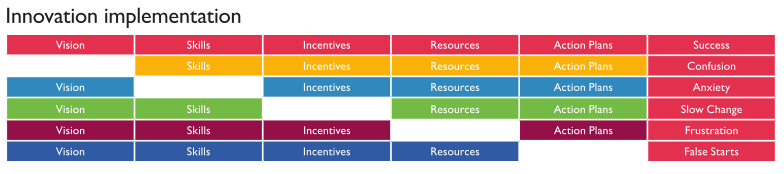
\includegraphics[scale=0.57]{figures/innovation-implementation}
	\caption{Five elements of successful change management and innovation implementation \citep{ADEC2016}, adapted from \cite{Thousand2001}}
\label{fig:implementation} 
\end{figure}

Given the preparation and planning that has gone into the SCF document, what ideas can we extract from this that would have improved the innovation introduction?

\begin{itemize}
	\item Context - the SCF places their version in the global context by comparing and contrasting with existing student frameworks and building upon them
	\item Timescale - from start to end, the process will take seven years, covering a pilot and monitoring phase
	\item Stakeholders - extensive work with stakeholders before and during the process to identify problems and opportunities
	\item Support - one the planned tasks for ensuring buy-in is: "developing appropriate guidance and support materials"
\end{itemize}

The SCF is a larger project than the innovation addition, but "too many good initiatives have failed through limiting their roll-out strategies to a dissemination of information \citep{Cordingley2007}" \citep{ADEC2016}.

\subsubsection{Innovation Guide}
A common theme during this research process was the slight confusion and hesitation towards implementation at the very start of the process due to the lack of guidance initially, and the fact there had not been any feedback from inspections. A publication was discovered entitled "A Guide to Development and Promotion of Innovation Skills" by ADEC \citet{ADEC2015a}. This document does not appear online anywhere  at all, and while is it referenced in an online newsletter, no digital version appears to exist. Requests to ADEC for a soft copy went unanswered, so the guide is included as Appendix \ref{appendix:adec}.\footnote{https://www.adec.ac.ae/en/MediaCenter/Publications/Teaching\%20Matters\%20Newsletter-Issue\%2017/files/assets/common/downloads/publication.pdf} A straw poll survey of schools indicate that they did not receive a copy of this, but this could not be confirmed across all schools. This document addresses a lot of problems with how innovation is defined, framed and assessed, it is unclear why it has not been either made available, or more readily accessible given its content. There are several areas worth highlighting in the document.

The stated aim of the guide is to ``offer a range of ideas and suggestions that schools adapt and use to suit their circumstances" \cite[p. 3]{ADEC2015a}. This is clearly the resource that teachers and schools  have stated they thought they were lacking.

Discussing innovation skills, the guide expands them into `imagination and creativity' and `critical thinking and problem solving'. Both are almost the same as the skills that the research and teachers have been using and discussing.

Where the guide really excels, and in fact provides more detail than even the inspection framework on measuring innovation standards. Shown in Figures \ref{fig:measuring-innovation} and \ref{fig:innovation-examplar} are snippets of detailed accounts of how to measure and to teach innovation skills. Interestingly, all the exemplars given are for primary schools, indicating that this may have been prepared specifically for primary schools.

\begin{figure}[h]
	\centering
	\captionsetup{justification=centering}
	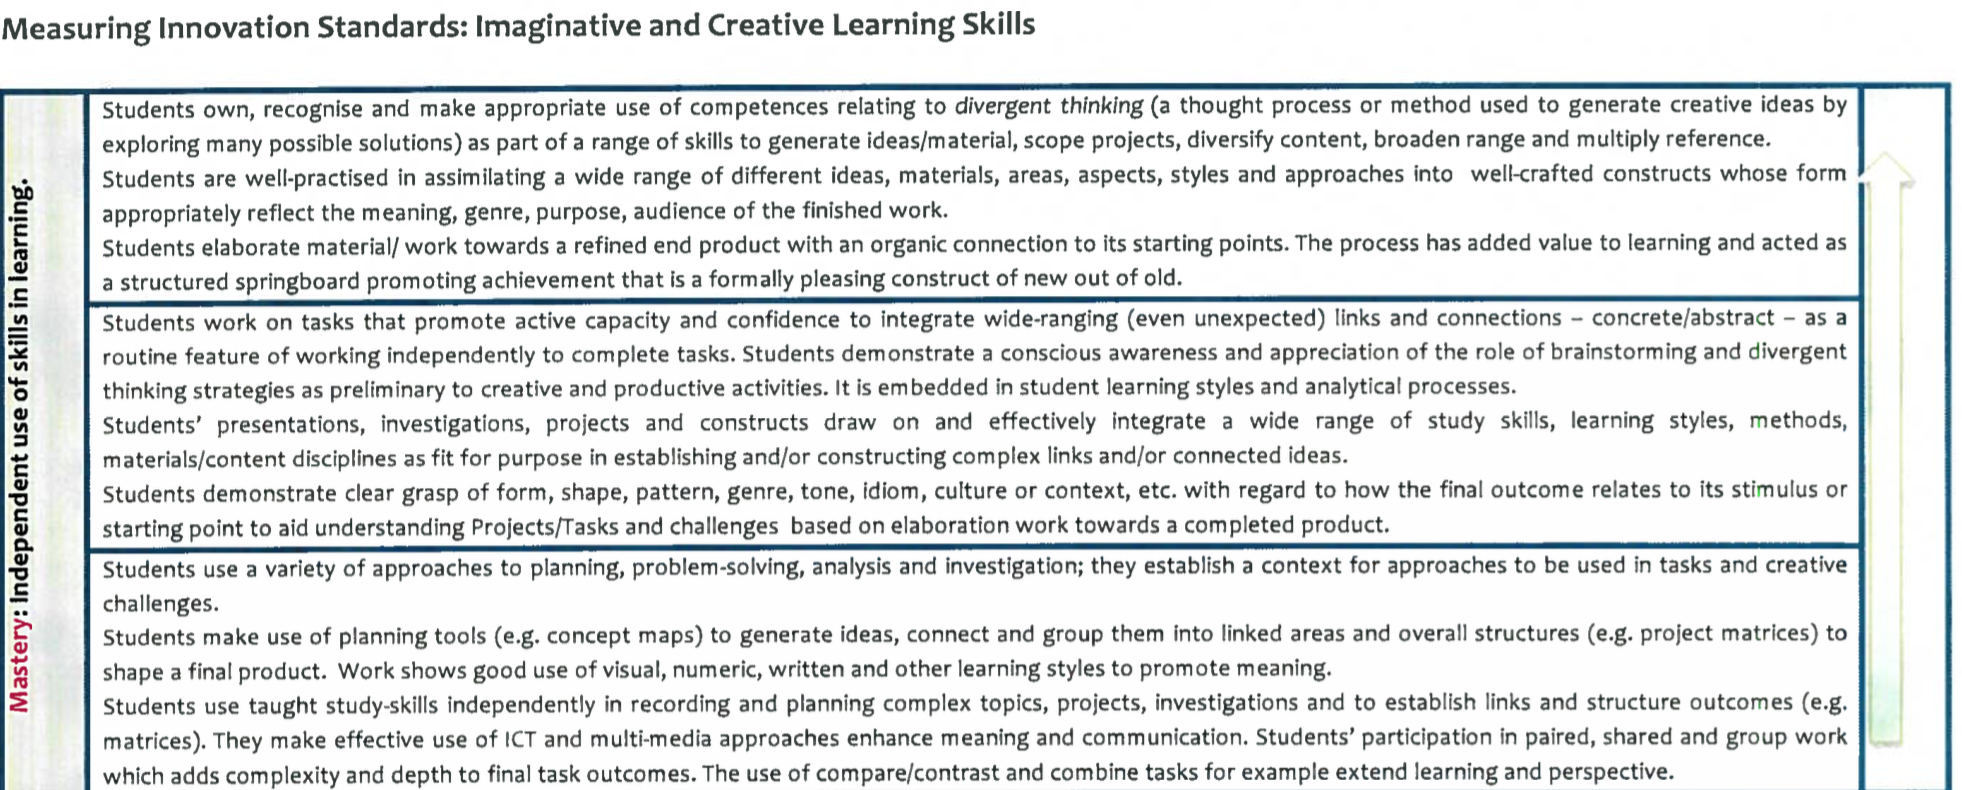
\includegraphics[scale=0.5]{figures/measuring-innovation}
	\caption{An excerpt of a guide on how to measure innovation skills  \citep[p. 19]{ADEC2015a}}
	\label{fig:measuring-innovation} 
\end{figure}

\begin{figure}[h]
	\centering
	\captionsetup{justification=centering}
	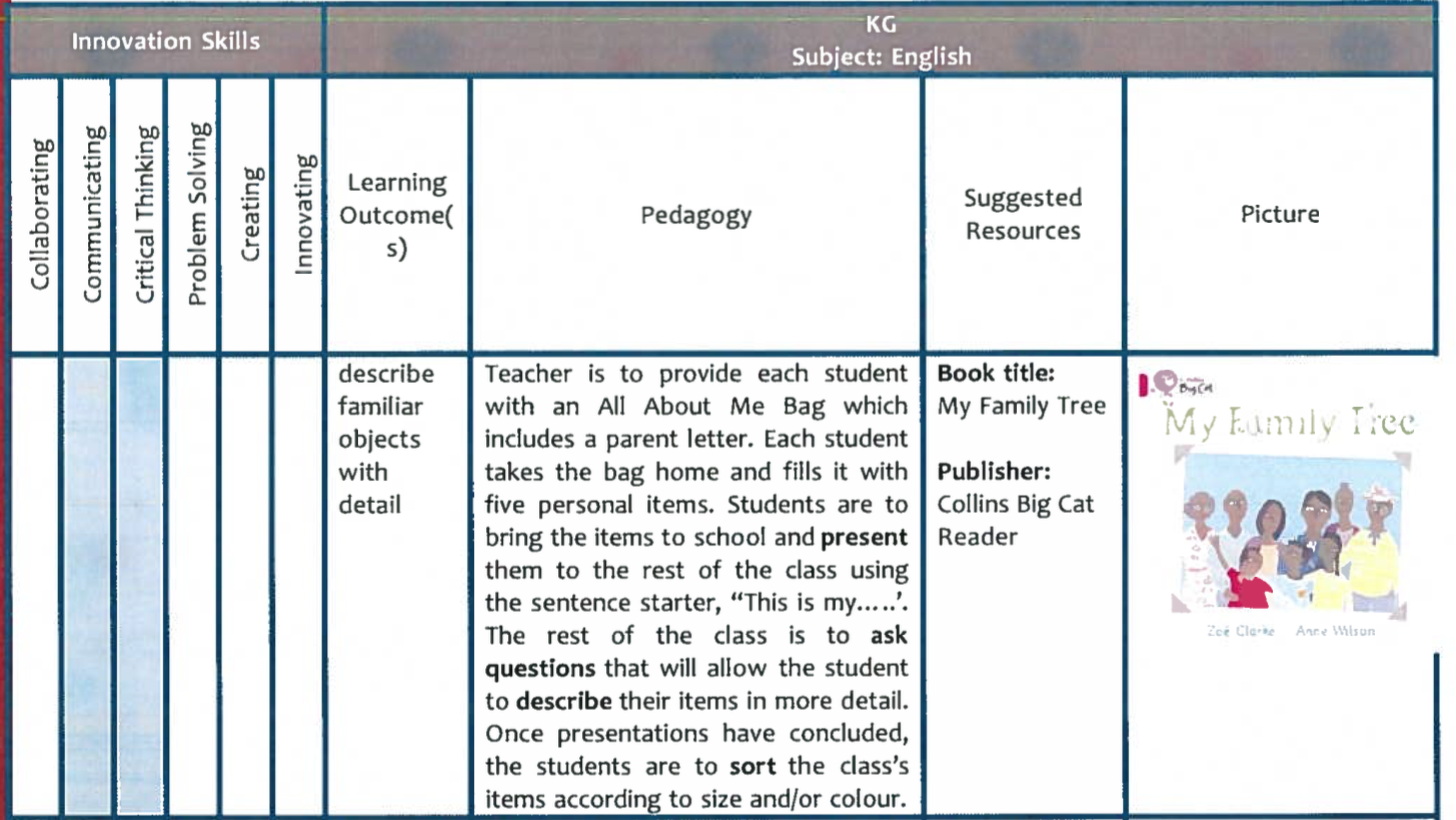
\includegraphics[scale=0.6]{figures/innovation-examplar}
	\caption{An exemplar for teaching innovation skills  \citep[p. 25]{ADEC2015a}}
	\label{fig:innovation-examplar} 
\end{figure}

\subsubsection{ADEC Curriculum Changes}
Almost too late to be of note for this research, ADEC announced it was making sweeping changes to its public school curriculum \cite{WAM1}. In the press release, ADEC stated that students would be commencing study of a compulsory subject called `Digital Technology and Innovation'. In the literature review there was a discovery of an Innovation Studies subject, but this was based on Design \& Technology whereas this press release seems to imply it is closer to ICT or Computer Science.

A similar press release was also released by the ruler of Dubai with slightly more detail on the plans \cite{WAM2}. This press release details that  the``new curriculum will cover technology[and] innovative design...'. There is also going to be a focus on ``building their critical thinking and innovation skills as well as developing teamwork and problem solving capabilities using innovative information and communication technology''. 

From the latter press release, it seems less likely that innovation will be a subject in itself. It does however, seem be a crucial part of a more advanced and forward-thinking IT-based subject, with a large focus on cross-curricular innovation skills.

Given the prevalence of private schools, it remains to be seen how much of an impact these changes will make on the county's education as a whole. An issue that was preciously discussed in this study.

\theendnotes
\section{Chapter 6}
\subsection{Conclusions and recommendations}
Abu Dhabi and the UAE have set out to drive forward its education system by way of making it more innovative. The focus on innovation within the UAE's society was included as an important facet of their UAE 2021 Vision document \citep{UAEGovernment2012}. In order for the UAE to produce more innovative citizens, the obvious consequence was to include this as a component of the education system. It was included as a relatively large component of the UAE unified inspection framework for the academic year 2015-2016.

In the first instance, there was an initial surprise to the addition from schools, a reaction which was discovered through observations and interviews. While educational themes and foci come and go with regularity, the focus on something as abstract as innovation along with its prominence made this different.

For many schools, a defensive reaction to this was for many schools to plan innovation days or weeks early in the 2015-2016 academic year. Some did this proactively, but many did so in response to an announced Emirate-wide innovation week from 22nd to 28th November. 

The innovation weeks highlighted two problems that would become evident at other times: it was announced with short notice and as a result, it conflicted with many schools' academic plans, including internal and external exams.
Early on in the process, it highlighted that innovation takes adequate planning, as well as the fact it can often conflict with daily school life if arranged as an off-timetable day or week.

Observations and interviews reflecting on this time showed a great deal of uncertainty, especially those schools who were due to be inspected that academic year. Defining innovation and identifying suitable examples was the first challenge within schools. The innovation week, while short notice, did provide an indication that showcasing innovative teaching and learning opportunities would be the focus of ADEC and its inspectors.

During the research, a range of teachers were interviewed and a few schools were chosen for closer examination in the form of a case study. This was combined with observations of the impact felt in the schools themselves.

After a few terms of including innovation in the framework, teachers could provide reasonably clear definitions of what innovation is. These definitions matched closely to those given in the literature. The definitions fell into two general categories: those that discussed innovation with respect to teaching and learning, and those that expressed more general definitions of innovation as a whole-school process.

This still indicates that while innovation is understood as a principle, there are multiple strands of innovation that while fall under the umbrella definition which look very different in practice. Those definitions referring to whole-school innovation did also not come from solely management roles as might have been expected.

It is not a surprise that the strands of innovation in education have become conflated. As discussed, innovation is a process which can be applied to many areas. Indeed, ADEC itself provided eight categories of possible innovation, many of those containing multiple smaller categories themselves.

When looking at case studies of schools which were above average in terms of innovation, it became clear that the more innovative schools are tackling many of the strands and that innovation is a school focus which begins with the leadership team and disseminated effectively throughout the school. There were many methods of doing this, including: giving staff time or money to focus on discovery of innovative ideas or pilot schemes; encouragement or allowances to facilitate greater collaboration with an aim at innovative learning events and a focus on innovation within teaching and learning.

It is very difficult, if not impossible, to become an innovative school, or to produce innovative schools without a focus and change in priorities at, or near, the top of a school leadership structure. This can be seen in inspection reports, by comparing schools which have been praised for being innovative and those that have been singled out as weak. As already discussed, innovation at a micro level can often lead to failure. If there is not a culture of trust wherein teachers are not worried about failing when innovating, it cannot succeed at the macrocosmic, whole-school (or wider) level.

There was also an element of experimentation and action research seen, which is not surprising if innovation is considered in a systematic way by trying and evaluation multiple ideas and projects to rapidly iterate to find the better ideas. This is promising if we are to take the Finnish model as one that could be replicated. Finland's intensive five-year teaching qualification is heavily focused on producing teachers for whom educational theory and research is an utmost priority. 

Outside of the schools themselves, it was clear from the literature that the innovation focus is here to stay, with it forming part of the national agenda. This brought up a few opportunities as well as a few challenges.

As a relatively young country and along with the governance structure and emphasis on education, the foundation of becoming an innovative education on a global level is there. Parallels with the Finnish education system were drawn, especially in terms of social and industrial development. One major difference, and one highlighted in the development of the Finnish model was the lack of cultural diversity within the country, which albeit had increased rapidly during this time. The cultural diversity in the UAE is rightfully seen as a cultural and social success, it does however lead to additional challenges in gaining any consistency within teaching standards. The teaching body consists of teachers from many different countries and this results in inherent differences in qualifications standards.

This is highlighted by one of the outcomes from the case studies: innovation works best when built on a foundation of solid teaching and learning. For all the strides the UAE has made in recent years, its education is still ranked as 46th out of 65 based on the 2012 PISA rankings \citep{2013}. They are however, aiming for top 20 by 2021 \citep{UAEGovernment2012}.

One of the problems identified in UAE public schools is the use of rote teaching practices and teaching from textbooks \cite[p. 88]{hatherley2012cultural} . This is substantiated by an interview by a director of the Organisation of Economic Co-operation and Development (OECD), the organisation who administer the PISA tests. He explains that the UAE is "way below" expectations \citep{Navdar2016}, mainly because of the lack of creative thinking from students. 

An innovation drive is therefore a good solution to close this gap, but without a solid teaching and learning platform and foundation, innovation can fall short and could even exacerbate the problem for some schools.

The lack of a central control curriculum is also an additional threat posed to a successful innovation drive. In theory, the curriculum shouldn't dictate how innovative a school can be, but those schools who are restricted to inflexible curriculum models can start the process at an immediate disadvantage. One of Finland's reasons for a successful and innovative education system was the removal of their inflexible curriculum and afforded greater flexibility for curricula to schools \citep{Simola2005}. One of the ostensible advantages of schools in Abu Dhabi is the ability to choose from multiple curricula, British, American, French, Japanese, Indian and local curricula comprise the majority of schools. This enables families in a transient country to choose a school curriculum that is either familiar to them, or one that will provide continuity if they regularly move or if students are aiming for university. The advantage can also prove a disadvantage when trying to enforce consistency (or flexibility) and a common direction when schools are restricted to their national curriculum.

Innovative teaching is often seen as the antithesis to rote-style learning but many of the curricula are still reliant on it, primarily due to the prominence, amount or form of formal assessments. This reflects the greater educational conundrum of trying to teach a wide and engaging curriculum while being assessed as a school on their national examination results. Quite how much pressure and expectation is placed on international schools compared to their local counterparts is outside the scope of this research but could play a factor in how well the innovation drive performs.

As a project in itself, aiming to create an innovative education system is by definition innovative. The introduction of the SCF late in the academic year provided an interesting addendum to the entire process. The SCF goes hand-in-hand with the existing innovation drive and it provides a blueprint for change management of innovative projects. This blueprint could be equally applied to SCF, school projects and the innovation drive.

It is hard to convincingly argue that the inclusion of the innovation framework is the same size as the SCF project, and therefore would benefit from being treated in the same manner. However, once we compare the issues raised by teachers and schools during the first year with the research in the SCF document the justification becomes a bit stronger.

Using t	he innovation implementation shown in Figure \ref{fig:implementation}, it indicated that there was a lack of clear vision for the innovation drive. Without confirmation, it can only be speculated that the SCF is a sister project  of the innovative drive, something which falls underneath it as a strand, or a replacement.

The inclusion of innovation within the unified framework is a solid idea, with it seemingly addressing a real need in helping the UAE achieve a better education and industry. It has been shown that a clearer vision would have helped prevent the initial confusion, specifically some context or global comparisons would have helped schools, the SCF project has done that in a completely thorough manner.

The UAE's development of education in the previous decade has been rapid and mostly successful, although signs of cohesion are emerging, there is still a way to go to achieve any standard of consistency. The diversity of educational establishments has been both an advantage to its large expatriate community for choice, as well as potential challenge to the government to ensure foci such as this one provide the greatest impact.

The relative disparity in the standard of teaching from the worst to the best schools is still large. It was indicated that innovation would have the most impact on the better schools. This may lead to a negative opinion of innovation in other schools, wherein it could become a stick rather than a carrot; an extra burden rather than a positive mentality for change.

The UAE has all the components it needs to create a world-class education system in the same way Dubai has become the global city in terms of tourism and property and retail development. The national agenda of innovation is a clear path to address its current problems with its underperforming education system. While it is still early, many schools have reacted positively which has already been observed by school inspection teams.

Ultimately it will be up to schools themselves whether innovation can become permeated within the fabric of their institutions as a driving force for cutting edge education, or whether it will be wheeled out for inspectors only to put it back in the cupboard to gather dust until the next inspection.

\bibliography{bibliography/biblio}


\begin{appendices}
	\section{Teacher Survey}
	\label{appendix:teachersurvey}
    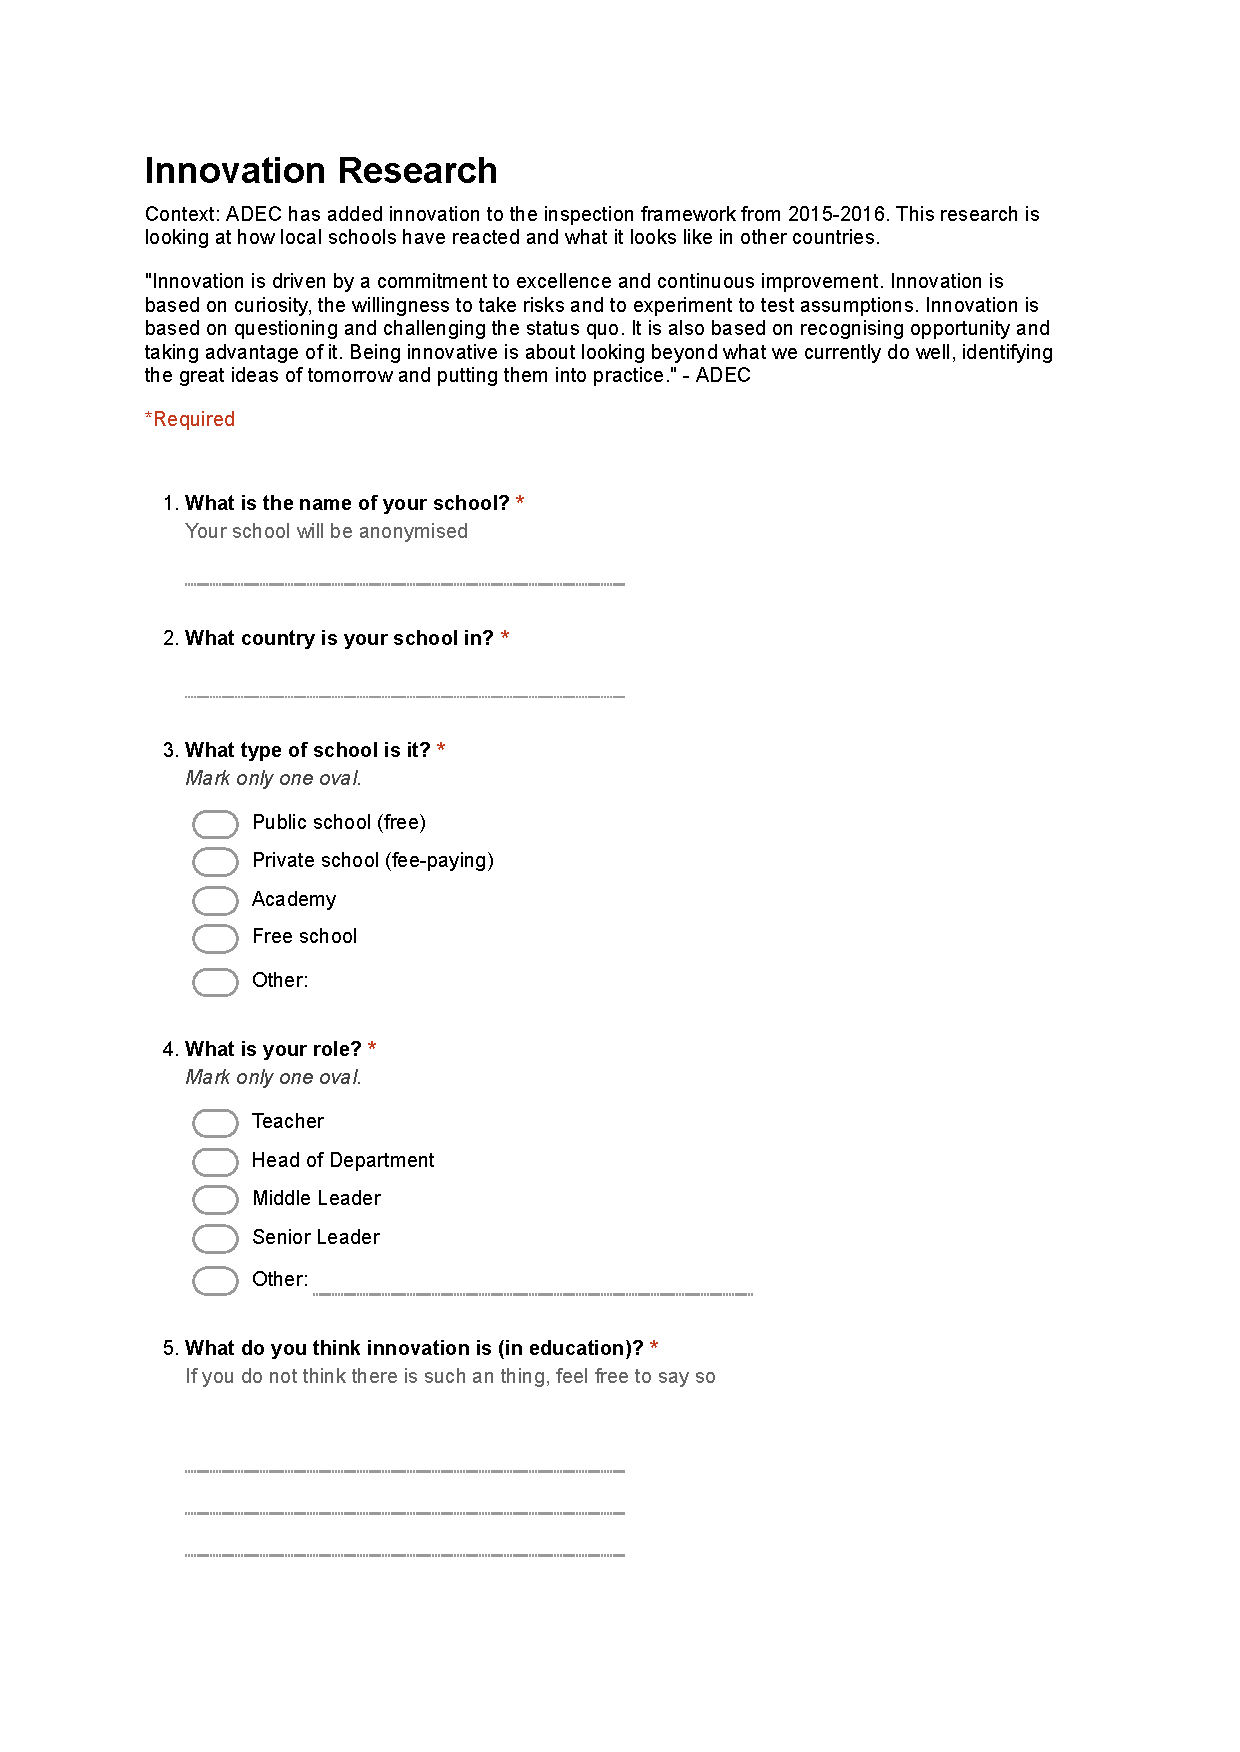
\includepdf{TeachersForm}
	
	\section{ADEC's `A Guide to Development and Promotion of Innovation Skills'}
	\label{appendix:adec}
	\includepdf[pages=-]{ADECInnovationGuide}
	
\end{appendices}

\end{document}

